\documentclass[dvips]{foils}
%\documentclass[dvips, french]{slides}
\textwidth 18.5cm
\textheight 25cm 
\topmargin -1cm 
\oddsidemargin  -1cm 
\evensidemargin  -1cm

% Maths
\usepackage{amsfonts, amsmath, amssymb, url}

\newcommand{\coefbin}[2]{\left( 
    \begin{array}{c} #1 \\ #2 \end{array} 
  \right)}
\newcommand{\bbullet}{\bullet\bullet}
\newcommand{\bbbullet}{\bbullet\bullet}
\newcommand{\bbbbullet}{\bbbullet\bullet}
\newcommand{\Bcal}{\mathcal{B}}
\newcommand{\Ccal}{\mathcal{C}}
\newcommand{\Dcal}{\mathcal{D}}
\newcommand{\Ecal}{\mathcal{E}}
\newcommand{\Fcal}{\mathcal{F}}
\newcommand{\Gcal}{\mathcal{G}}
\newcommand{\Mcal}{\mathcal{M}}
\newcommand{\Ncal}{\mathcal{N}}
\newcommand{\Pcal}{\mathcal{P}}
\newcommand{\Qcal}{\mathcal{Q}}
\newcommand{\Rcal}{\mathcal{R}}
\newcommand{\Hcal}{\mathcal{H}}
\newcommand{\Jcal}{\mathcal{J}}
\newcommand{\Lcal}{\mathcal{L}}
\newcommand{\Tcal}{\mathcal{T}}
\newcommand{\Ucal}{\mathcal{U}}
\newcommand{\Xcal}{\mathcal{X}}
\newcommand{\Zcal}{\mathcal{Z}}
\newcommand{\dd}{\text{d}}
\newcommand{\etabar}{\overline{\eta}}
\newcommand{\pibar}{\overline{\pi}}
\newcommand{\alphabf}{\mbox{\mathversion{bold}{$\alpha$}}}
\newcommand{\betabf}{\mbox{\mathversion{bold}{$\beta$}}}
\newcommand{\gammabf}{\mbox{\mathversion{bold}{$\gamma$}}}
\newcommand{\mubf}{\mbox{\mathversion{bold}{$\mu$}}}
\newcommand{\nubf}{\mbox{\mathversion{bold}{$\nu$}}}
\newcommand{\phibf}{\mbox{\mathversion{bold}{$\phi$}}}
\newcommand{\pibf}{\mbox{\mathversion{bold}{$\pi$}}}
\newcommand{\Pibf}{\mbox{\mathversion{bold}{$\Pi$}}}
\newcommand{\psibf}{\mbox{\mathversion{bold}{$\psi$}}}
\newcommand{\Sigmabf}{\mbox{\mathversion{bold}{$\Sigma$}}}
\newcommand{\taubf}{\mbox{\mathversion{bold}{$\tau$}}}
\newcommand{\thetabf}{\mbox{\mathversion{bold}{$\theta$}}}
\newcommand{\Abf}{{\bf A}}
\newcommand{\Ebf}{{\bf E}}
\newcommand{\Hbf}{{\bf H}}
\newcommand{\Ibf}{{\bf I}}
\newcommand{\Obf}{{\bf 0}}
\newcommand{\Sbf}{{\bf S}}
\newcommand{\mbf}{{\bf m}}
\newcommand{\ubf}{{\bf u}}
\newcommand{\vbf}{{\bf v}}
\newcommand{\xbf}{{\bf x}}
\newcommand{\Xbf}{{\bf X}}
\newcommand{\ybf}{{\bf y}}
\newcommand{\Zbf}{{\bf Z}}
\newcommand{\Esp}{{\mathbb E}}
\newcommand{\ERMG}{\text{Mix}}
\newcommand{\Corr}{{\mathbb C}\mbox{orr}}
\newcommand{\Nbb}{\mathbb{N}}
\newcommand{\Nm}{N(\mbf)}
\newcommand{\mum}{\mu(\mbf)}
\newcommand{\obs}{\text{obs}}
\newcommand{\Ibb}{{\mathbb I}}
\newcommand{\Omegas}{\underset{s}{\Omega}}
\newcommand{\Var}{{\mathbb V}}
\newcommand{\Pro}{\mathbb{P}}
\newcommand{\Rbb}{\mathbb{R}}
\newcommand{\RX}{R_{\Xbf}}
\newcommand{\Vsf}{\mathsf{V}}
\newcommand{\Starsf}{\mathsf{*}}
\newcommand{\QZ}{Q_{\Zbf}}
\newcommand{\QZi}{Q_{\Zbf_i}}
\newcommand{\Qt}{Q_{\thetabf}}


% Couleur et graphiques
\usepackage{color}
\usepackage{graphics}
\usepackage{epsfig} 
\usepackage{pstcol}

% Texte
\usepackage{lscape}
\usepackage{../../../../Latex/fancyheadings, rotating, enumerate}
%\usepackage[french]{babel}
\usepackage[latin1]{inputenc}
%\definecolor{darkgreen}{cmyk}{0.5, 0, 0.5, 0.5}
%\definecolor{green}{cmyk}{0.5, 0, 0.5, 0.5}
\definecolor{orange}{cmyk}{0, 0.6, 0.8, 0}
\definecolor{jaune}{cmyk}{0, 0.5, 0.5, 0}
\newcommand{\textblue}[1]{\textcolor{blue}{#1}}
\newcommand{\textred}[1]{\textcolor{red}{#1}}
\newcommand{\textgreen}[1]{\textcolor{green}{ #1}}
\newcommand{\textlightgreen}[1]{\textcolor{green}{#1}}
%\newcommand{\textgreen}[1]{\textcolor{darkgreen}{#1}}
\newcommand{\textorange}[1]{\textcolor{orange}{#1}}
\newcommand{\textyellow}[1]{\textcolor{yellow}{#1}}
\newcommand{\emphase}[1]{\textblue{\sl #1}}
\newcommand{\refer}[1]{\textgreen{\sl #1}}

% Sections
%\newcommand{\chapter}[1]{\centerline{\LARGE \textblue{#1}}}
% \newcommand{\section}[1]{\centerline{\Large \textblue{#1}}}
% \newcommand{\subsection}[1]{\noindent{\Large \textblue{#1}}}
% \newcommand{\subsubsection}[1]{\noindent{\large \textblue{#1}}}
% \newcommand{\paragraph}[1]{\noindent {\textblue{#1}}}
% Sectionsred
\newcommand{\chapter}[1]{
  \addtocounter{chapter}{1}
  \setcounter{section}{0}
  \setcounter{subsection}{0}
  {\centerline{\LARGE \textblue{\arabic{chapter} - #1}}}
%  {\centerline{\LARGE \textblue{#1}}}
  }
\newcommand{\section}[1]{
  \addtocounter{section}{1}
  \setcounter{subsection}{0}
  {\noindent {\Large \textblue{\arabic{chapter}.\arabic{section} - #1}}}
%  {\noindent {\Large \textblue{#1}}}
  }
\newcommand{\subsection}[1]{
  \addtocounter{subsection}{1}
%   {\noindent{\large
%       \textblue{\arabic{chapter}.\arabic{section}.\arabic{subsection}
%         - #1}}}
  {\noindent{\large \textblue{#1}}}
  }
\newcommand{\paragraph}[1]{\noindent{\textblue{#1}}}

%%%%%%%%%%%%%%%%%%%%%%%%%%%%%%%%%%%%%%%%%%%%%%%%%%%%%%%%%%%%%%%%%%%%%%
%%%%%%%%%%%%%%%%%%%%%%%%%%%%%%%%%%%%%%%%%%%%%%%%%%%%%%%%%%%%%%%%%%%%%%
%%%%%%%%%%%%%%%%%%%%%%%%%%%%%%%%%%%%%%%%%%%%%%%%%%%%%%%%%%%%%%%%%%%%%%
%%%%%%%%%%%%%%%%%%%%%%%%%%%%%%%%%%%%%%%%%%%%%%%%%%%%%%%%%%%%%%%%%%%%%%
\begin{document}
%%%%%%%%%%%%%%%%%%%%%%%%%%%%%%%%%%%%%%%%%%%%%%%%%%%%%%%%%%%%%%%%%%%%%%
%%%%%%%%%%%%%%%%%%%%%%%%%%%%%%%%%%%%%%%%%%%%%%%%%%%%%%%%%%%%%%%%%%%%%%
%%%%%%%%%%%%%%%%%%%%%%%%%%%%%%%%%%%%%%%%%%%%%%%%%%%%%%%%%%%%%%%%%%%%%%
%%%%%%%%%%%%%%%%%%%%%%%%%%%%%%%%%%%%%%%%%%%%%%%%%%%%%%%%%%%%%%%%%%%%%%
\landscape
\newcounter{chapter}
\newcounter{section}
\newcounter{subsection}
\setcounter{chapter}{0}
\headrulewidth 0pt 
\pagestyle{fancy} 
\cfoot{}
\rfoot{\begin{rotate}{90}{
      \hspace{1cm} \tiny S. Robin: Uncovering structure in networks  
      }\end{rotate}}
\rhead{\begin{rotate}{90}{
      \hspace{-.5cm} \tiny \thepage
      }\end{rotate}}

%%%%%%%%%%%%%%%%%%%%%%%%%%%%%%%%%%%%%%%%%%%%%%%%%%%%%%%%%%%%%%%%%%%%%%
%%%%%%%%%%%%%%%%%%%%%%%%%%%%%%%%%%%%%%%%%%%%%%%%%%%%%%%%%%%%%%%%%%%%%%
\begin{center}
  \textblue{\LARGE Uncovering (global) structure}
  \\~\\
  \textblue{\LARGE and (local) motifs in networks}
  ~\\~\\~\\
  \textblue{\large St�phane Robin} \\
  {\tt robin@agroparistech.fr} \\
  ~\\~\\
  AgroParisTech / INRA, Paris \\
%   UMR 518 Math�matique et Informatique Appliqu�es \\
%   \url{www.agroparistech.fr/mia/} \\
  ~\\
  {Statistics for Biological Sequences (SSB) group} \\
%   \url{genome.jouy.inra.fr/ssb/} \\
  ~\\~\\
  \textblue{Joint work with J.-J. Daudin, M. Mariadassou, M. Koskas,
    F. Picard, S. Schbath} \\
  ~\\~\\
  \begin{tabular}{ccccc}
    
\epsfig{file=../Figures/LogoINRA-Couleur.ps, width=5cm} &
    \hspace{2cm} &
    
\epsfig{file=../Figures/logagroptechsolo.eps, width=7.5cm} &
    \hspace{2cm} &
    \epsfig{file=../Figures/Logo-SSB.eps, width=5cm} \\
  \end{tabular} \\
\end{center}

%%%%%%%%%%%%%%%%%%%%%%%%%%%%%%%%%%%%%%%%%%%%%%%%%%%%%%%%%%%%%%%%%%%%%
\newpage
\subsection{Outline}

\bigskip\bigskip\bigskip
\begin{tabular}{ll}
\emphase{Introduction}  & 1 - Some statistical issues in network
analysis \\
\\
& 2 - Looking for structure in networks \\
\\
\hline
\\
\emphase{Global structure} & 3 - Mixture model for random graphs \\
\\
& 4 - Variational inference \\
\\
\hline
\\
\emphase{Local structure} & 5 - Motifs in interaction graphs \\
\\
& 6 - Approximate distribution for the count \\
\\
\hline
\\
& 7 - Discussion \& Work in progress \\
\end{tabular}

%%%%%%%%%%%%%%%%%%%%%%%%%%%%%%%%%%%%%%%%%%%%%%%%%%%%%%%%%%%%%%%%%%%%%
%%%%%%%%%%%%%%%%%%%%%%%%%%%%%%%%%%%%%%%%%%%%%%%%%%%%%%%%%%%%%%%%%%%%%
\newpage
\chapter{Some statistical issues}
%%%%%%%%%%%%%%%%%%%%%%%%%%%%%%%%%%%%%%%%%%%%%%%%%%%%%%%%%%%%%%%%%%%%%
%%%%%%%%%%%%%%%%%%%%%%%%%%%%%%%%%%%%%%%%%%%%%%%%%%%%%%%%%%%%%%%%%%%%%

% %%%%%%%%%%%%%%%%%%%%%%%%%%%%%%%%%%%%%%%%%%%%%%%%%%%%%%%%%%%%%%%%%%%%%
% \bigskip
% \section{}
% %%%%%%%%%%%%%%%%%%%%%%%%%%%%%%%%%%%%%%%%%%%%%%%%%%%%%%%%%%%%%%%%%%%%%
\noindent
\begin{tabular}{cc}
  \begin{tabular}{p{12cm}}
    \section{Networks} \dots
    \begin{itemize}
    \item Arise in many fields:
      \begin{itemize}
      \item[\bf{$\rightarrow$}] Biology, Chemistry
      \item[\bf{$\rightarrow$}] Physics, Internet.
      \end{itemize}
    \item Represent an interaction pattern:
      \begin{itemize}
      \item[\bf{$\rightarrow$}] $\mathcal{O}(n^2)$ interactions
      \item[\bf{$\rightarrow$}] between $n$ elements.
      \end{itemize}
    \item Have a topology which:
      \begin{itemize}
      \item[\bf{$\rightarrow$}] reflects the structure / function
        relationship
      \end{itemize}
    \end{itemize}
  \end{tabular}
  &
  \begin{tabular}{c}
    \psfig{file=../Figures/caida2_lg(brown).ps, angle=270, width=11cm} \\
    \begin{tiny} From Barab\'asi website \end{tiny}
  \end{tabular}
\end{tabular}

%%%%%%%%%%%%%%%%%%%%%%%%%%%%%%%%%%%%%%%%%%%%%%%%%%%%%%%%%%%%%%%%%%%%
\newpage
\subsection{Some examples}

\paragraph{Social networks.}
\begin{itemize}
\item \vspace{-0.5cm} Who loves who? Who's friend with who?
\item \vspace{-0.5cm} Which covariates contribute to explain the
  existence of a link?
\end{itemize}
\paragraph{Industrial/commercial networks.}
\begin{itemize}
\item \vspace{-0.5cm} Number of passenger exchanged between airports.
\end{itemize}
\paragraph{Biological networks.}
\begin{itemize}
\item \vspace{-0.5cm} Which genes regulates which gene? Which proteins
  do interact?
\item \vspace{-0.5cm} Does it help in understanding their biological function?
\end{itemize} 
\paragraph{Internet.}
\begin{itemize}
\item \vspace{-0.5cm} How is growing? 
\item \vspace{-0.5cm} Do active website contain more relevant pieces
  of information?
\end{itemize}


%%%%%%%%%%%%%%%%%%%%%%%%%%%%%%%%%%%%%%%%%%%%%%%%%%%%%%%%%%%%%%%%%%%%
\newpage
\section{Statistical analysis}
%%%%%%%%%%%%%%%%%%%%%%%%%%%%%%%%%%%%%%%%%%%%%%%%%%%%%%%%%%%%%%%%%%%%%

%%%%%%%%%%%%%%%%%%%%%%%%%%%%%%%%%%%%%%%%%%%%%%%%%%%%%%%%%%%%%%%%%%%%
\subsection{A huge probabilistic literature ...}

Since the first works of \emphase{Erd�s \& R�nyi}, the
probabilistic properties of random graphs have been intensively
studied.

Typical quantities of interest are
\begin{itemize}
\item \vspace{-0.5cm} the number of connected components and the size
  of the largest one,
\item \vspace{-0.5cm} the node degrees (scale-free distribution?), 
\item \vspace{-0.5cm} the network diameter (small-world effect?),
\item \vspace{-0.5cm} the number of triangles and/or the clustering
  coefficient,
\item \vspace{-0.5cm} the spread of an epidemic or an innovation.
\end{itemize}
Numerous asymptotic and exact results are available, for large
classes of random graphs. \\
(see \refer{Pattison \& Robbins, 07} for a general review on random
graph models.)

%%%%%%%%%%%%%%%%%%%%%%%%%%%%%%%%%%%%%%%%%%%%%%%%%%%%%%%%%%%%%%%%%%%%
\newpage
\subsection{... But less in statistics}

Statistical tools to analyse network structured data seem to be much
more recent. \\ ~\\
\begin{tabular}{lc}
  Network data do not have the structure  &
  \emphase{individuals $\times$ variables} \\
  \\
  but rather &
  \emphase{individuals $\times$ individuals} \\
  \\
  or even &
  \emphase{individuals $\times$ individuals $\times$ variables}
\end{tabular}

\bigskip\bigskip
\paragraph{Some typical questions:}
\begin{itemize}
\item \vspace{-0.5cm} How to infer a network from data observed at
  each node?
\item \vspace{-0.5cm} How to fit a random graph model to an observed network?
\item \vspace{-0.5cm} How to predict the existence of an edge, or some
  characteristic of a node given its connexions to others?
\item \vspace{-0.5cm} ...?
\end{itemize}


%%%%%%%%%%%%%%%%%%%%%%%%%%%%%%%%%%%%%%%%%%%%%%%%%%%%%%%%%%%%%%%%%%%%
\newpage
\section{Network inference}
%%%%%%%%%%%%%%%%%%%%%%%%%%%%%%%%%%%%%%%%%%%%%%%%%%%%%%%%%%%%%%%%%%%%

\noindent Network are often used to depict dependencies (edges)
between entities (nodes).  Network inference aims to \emphase{estimate
  the dependency structure} from data observed at each node.

\paragraph{Graphical Gaussian models} provide a proper
statistical framework to achieve this inference: Denoting $\Xbf_j$ the
$n$-vector observed at replicate $j$, suppose
$$
\{\Xbf_j\}_{j=1..k} \text{ i.i.d. } \sim \Ncal_n(\mubf, \Sigmabf).
$$
\paragraph{Dynamic Bayesian networks} provide an alternative
for dynamic data: Denoting $\Xbf_t$ the $n$-vector observed at time
$t$, suppose
$$
\Xbf_{t+1} = \Abf \Xbf_t + \Ebf_{t+1}, \qquad \{\Ebf_t\} \text{ i.i.d. }
\sim \Ncal_n(\Obf, \sigma^2 \Ibf).
$$

\paragraph{Goal:} Estimate $\Sigmabf$ or $\Abf$ and the \emphase{set
  of their non-zero coefficients}.

%%%%%%%%%%%%%%%%%%%%%%%%%%%%%%%%%%%%%%%%%%%%%%%%%%%%%%%%%%%%%%%%%%%%%
\newpage
\subsection{Statistical issues}

\paragraph{Non-stationary data.} The i.i.d. or ergodicity hypotheses
are often violated.

\paragraph{'$p \gg n$' paradigm.} The number of observations
(replicates, dates) is generally much smaller than the number of
variables (nodes).
\begin{enumerate}[$\rightarrow$]
\item \vspace{-0.5cm} Partial correlation coefficient are more
  relevant to describe direct links
\item \vspace{-0.5cm} Regularised (LASSO, shrinked) estimate of $\Sigmabf^{-1}$
\end{enumerate}

\paragraph{Multiple testing.} 
\begin{enumerate}[$\rightarrow$]
\item \vspace{-0.5cm} Immediately arise when testing for the existence
  of each edge
\item \vspace{-0.5cm} Shrinkage estimates + multiple testing
  (\emphase{see 2nd talk})
\end{enumerate}


%%%%%%%%%%%%%%%%%%%%%%%%%%%%%%%%%%%%%%%%%%%%%%%%%%%%%%%%%%%%%%%%%%%%
\newpage
\section{Fitting a random graph model}
%%%%%%%%%%%%%%%%%%%%%%%%%%%%%%%%%%%%%%%%%%%%%%%%%%%%%%%%%%%%%%%%%%%%%

Many random graph models have been proposed, involving several
parameters.

\begin{tabular}{cc}
  \hspace{-2.2cm}
  \begin{tabular}{p{14cm}}
    \paragraph{Preferential attachment:} (dynamic model) \\
    $\rightarrow$ mean number of connexion of a new node, influence of
    the degree  \\ ~\\ ~\\
    % (\refer{Barabasi \& al., 04}) 
  \end{tabular}
  &
  \begin{tabular}{p{10cm}}
    \centerline{
%       \epsfig{file=../Figures/Barabasi4.ps, width=5cm, height=4cm,
%         bbllx=383, bblly=470, bburx=585, bbury=660, clip=}
    \epsfig{file=../Figures/FigNetworks-PrefAtt-Col.eps, width=5cm,
      height=4cm}
      }
  \end{tabular}
\end{tabular} \\
\begin{tabular}{cc}
  \hspace{-1.2cm}
  \begin{tabular}{p{14cm}}
  \paragraph{Duplication / Deletion:} (dynamic model): \\
  $\rightarrow$ duplication probability, deletion probability. \\
  (pict. from \refer{Ratman \& al., 07}) \\ ~\\ ~\\ ~\\
  \end{tabular}
  &
  \begin{tabular}{p{10cm}}
    \centerline{
                                % RJH07-PLoSCompBiol.pdf
      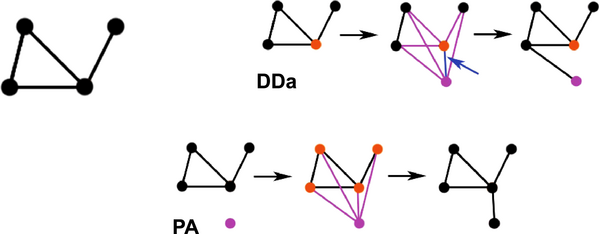
\epsfig{file=../Figures/RJH07-PLoSCompBiol-Fig7.ps, width=9cm,
        height=4cm, bbllx=255, bblly=150, bburx=580, bbury=240, clip=}
      }
  \end{tabular}
\end{tabular} \\
\paragraph{Exponential random graph models:} (ERGM or
'$p^*$') \\
$\rightarrow$ expected value of some sufficient statistics

\paragraph{Mixture models:} \\
$\rightarrow$ group proportions, between-group connectivities.

%%%%%%%%%%%%%%%%%%%%%%%%%%%%%%%%%%%%%%%%%%%%%%%%%%%%%%%%%%%%%%%%%%%%%
\newpage
\subsection{Statistical inference}

\noindent Due to \emphase{very intricate dependencies} and to
\emphase{unobserved data} (e.g. historical), standard maximum
likelihood approaches often fail...
\begin{enumerate}[$\rightarrow$]
\item \vspace{-0.5cm} Stochastic approximations of E-M, 
\item \vspace{-0.5cm} Bayesian inference / MCMC algorithms, 
\item \vspace{-0.5cm} Likelihood-free methods / approximate Bayesian
  computing (ABC),
\item \vspace{-0.5cm} Variational approximations
  (\emphase{see 1st talk})
\end{enumerate}

\paragraph{Some open questions.}
\begin{itemize}
\item \vspace{-0.5cm} Statistical properties of the estimates.
\item \vspace{-0.5cm} Efficient algorithms for very large networks (internet).
\item \vspace{-0.5cm} \emphase{Finding the right model for a given question.}
\end{itemize}

%%%%%%%%%%%%%%%%%%%%%%%%%%%%%%%%%%%%%%%%%%%%%%%%%%%%%%%%%%%%%%%%%%%%
\newpage
\section{Classification / Prediction}
%%%%%%%%%%%%%%%%%%%%%%%%%%%%%%%%%%%%%%%%%%%%%%%%%%%%%%%%%%%%%%%%%%%%

Network data are sometimes partially observed:
\begin{itemize}
\item \vspace{-0.5cm} Missing links
\item \vspace{-0.5cm} Missing information on some nodes
\end{itemize}

Does the network structure help to predict the missing information?

\bigskip\bigskip
\subsection{Some strategies}

\paragraph{0/1 classification.} Predicting the existence of an edge is
a typical statistical learning problem.
\begin{itemize}
\item \vspace{-0.5cm} Standard models such as logistic regression can
  be used \\
  $\rightarrow$ the covariates are often observed on the nodes, while
  the response is on an edge.
\item \vspace{-0.5cm} Building a classifier for each node is a way to
  cope with this asymmetry.
\end{itemize}

%%%%%%%%%%%%%%%%%%%%%%%%%%%%%%%%%%%%%%%%%%%%%%%%%%%%%%%%%%%%%%%%%%%%
\newpage
\paragraph{Predicting the color of a node.} Suppose that each node has
a color (e.g. a biological function) and that this color is missing
for some of them.
\begin{itemize}
\item \vspace{-0.5cm} Nearest neighbour strategy can be considered.
\item \vspace{-0.5cm} Accounting for more complex topology may improve
  (\emphase{see 3rd talk})
\end{itemize}

%%%%%%%%%%%%%%%%%%%%%%%%%%%%%%%%%%%%%%%%%%%%%%%%%%%%%%%%%%%%%%%%%%%%
\newpage
\section{Dynamic behaviour}
%%%%%%%%%%%%%%%%%%%%%%%%%%%%%%%%%%%%%%%%%%%%%%%%%%%%%%%%%%%%%%%%%%%%

In the \emphase{complex systems} or \emphase{systems biology}
community, networks often describe a set of differential equations.
\begin{enumerate}[$\rightarrow$]
\item \vspace{-0.5cm} ODE / PDE / SDE modelling
\item \vspace{-0.5cm} Theoretical study of the systems (stable points, limit
  cycles, {\sl etc}.)
\item \vspace{-0.5cm} Parameter inference (\emphase{see invited
    session 8b ... on Tuesday})
\end{enumerate}

\paragraph{Personal question.} How to make inference with tens or
hundreds of compartments (nodes) ... and few replicates.

%%%%%%%%%%%%%%%%%%%%%%%%%%%%%%%%%%%%%%%%%%%%%%%%%%%%%%%%%%%%%%%%%%%%%
%%%%%%%%%%%%%%%%%%%%%%%%%%%%%%%%%%%%%%%%%%%%%%%%%%%%%%%%%%%%%%%%%%%%%
\newpage
\chapter{Looking for structure in networks}
%%%%%%%%%%%%%%%%%%%%%%%%%%%%%%%%%%%%%%%%%%%%%%%%%%%%%%%%%%%%%%%%%%%%%
%%%%%%%%%%%%%%%%%%%%%%%%%%%%%%%%%%%%%%%%%%%%%%%%%%%%%%%%%%%%%%%%%%%%%

%%%%%%%%%%%%%%%%%%%%%%%%%%%%%%%%%%%%%%%%%%%%%%%%%%%%%%%%%%%%%%%%%%%%%
%\newpage
\subsection{Global structure:} A simple example

\vspace{-2cm}
$$
\begin{tabular}{c}
  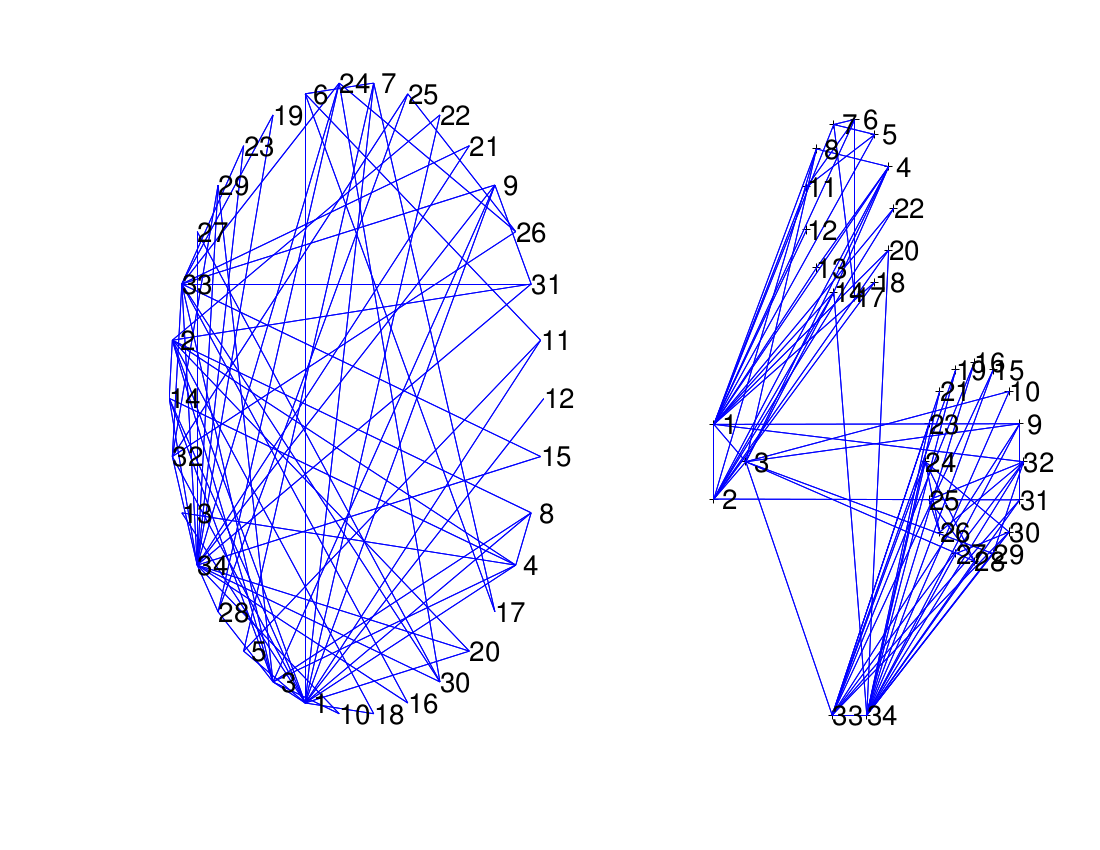
\epsfig{file = ../Figures/Karate-Graph.eps, clip=, width=7cm,
    height=20cm, angle=270}
  \\
  \epsfig{file = ../Figures/Karate-Dotplot.eps, clip=, width=7cm,
    height=20cm, angle=270}
\end{tabular}
$$

%%%%%%%%%%%%%%%%%%%%%%%%%%%%%%%%%%%%%%%%%%%%%%%%%%%%%%%%%%%%%%%%%%%%%
\newpage
\noindent
\begin{tabular}{cc}
  \begin{tabular}{p{15cm}}
    \subsection{Local structure:}\\
    \\
    \subsection{Patterns of interconnection} \\
    \\ \\
    \paragraph{Principle:} \\
    Break a complex network down \emphase{functional modules} to
    understand its behaviour.  \refer{Shen-Orr et al. (02)} \\    
    \\
    Such motifs may perform specific \emphase{regulatory functions}
    (e.g. feed-forward loop, bi-fan). \\
    \\
    They can be identified as \emphase{exceptional motifs}  i.e.
    motifs appearing \emphase{more frequently than expected}. 
    \\ \\ \\
  \end{tabular}
  &
  \begin{tabular}{c}
    \epsfig{file=../FIGURES/RegulationMotifs.ps, bbllx=82, bblly=89,
    bburx=289, bbury=600, clip=, height=16cm}
  \end{tabular}
\end{tabular}


%%%%%%%%%%%%%%%%%%%%%%%%%%%%%%%%%%%%%%%%%%%%%%%%%%%%%%%%%%%%%%%%%%%%%
%%%%%%%%%%%%%%%%%%%%%%%%%%%%%%%%%%%%%%%%%%%%%%%%%%%%%%%%%%%%%%%%%%%%%
\newpage
\chapter{Mixture model for random graphs}
%%%%%%%%%%%%%%%%%%%%%%%%%%%%%%%%%%%%%%%%%%%%%%%%%%%%%%%%%%%%%%%%%%%%%
%%%%%%%%%%%%%%%%%%%%%%%%%%%%%%%%%%%%%%%%%%%%%%%%%%%%%%%%%%%%%%%%%%%%%

%%%%%%%%%%%%%%%%%%%%%%%%%%%%%%%%%%%%%%%%%%%%%%%%%%%%%%%%%%%%%%%%%%%%
\section{Heterogeneity in networks}
%%%%%%%%%%%%%%%%%%%%%%%%%%%%%%%%%%%%%%%%%%%%%%%%%%%%%%%%%%%%%%%%%%%%%
~\\ ~\\ 
\centerline{\emphase{Nodes may have different connectivity behaviour.}}

\paragraph{Looking for connected sub-groups:}
\begin{itemize}
\item \vspace{-0.5cm} Detection of cliques or groups of highly
  connected nodes: \refer{Gethor \& Diehl, 04} 
\item \vspace{-0.5cm} Edge betweenness: \refer{Girvan \& Newman, 02}
\item \vspace{-0.5cm} Spectral clustering: \refer{Von Luxburg \& al.,
    07}
\end{itemize}

\paragraph{Model based:}
\begin{itemize}
\item \vspace{-0.5cm} Underlying topology: \refer{Hoff \& al., 02}
  (Latent space)
\item \vspace{-0.5cm} Mixture model \refer{Nowicki \& Snijders, 01}
  (Block structure), \refer{Daudin \& al., 08} (Mixture for graphs)
\item \vspace{-0.5cm} General model for heterogeneous networks:
  \refer{Bollob\'as \ al., 07} (Topological properties: Giant component,
  diameter, degree distribution = compound Poisson, {\it etc.}).
\end{itemize}

%%%%%%%%%%%%%%%%%%%%%%%%%%%%%%%%%%%%%%%%%%%%%%%%%%%%%%%%%%%%%%%%%%%%%
\newpage
\subsection{Random graph model}
%%%%%%%%%%%%%%%%%%%%%%%%%%%%%%%%%%%%%%%%%%%%%%%%%%%%%%%%%%%%%%%%%%%%%

We denote $i=1..n$ the \emphase{fixed nodes} and $X_{ij}$ the
\emphase{random edges}.

A random graph $G$ is completely characterised by $n$ and the
by the \emphase{joint distribution} of the $X_{ij}$'s.

The distribution of the degrees of the nodes is \emphase{not sufficient}.

\bigskip\bigskip
\paragraph{Classical models for binary graphs}
\begin{itemize}
\item \vspace{-0.5cm} \paragraph{Erd�s-R�nyi:} The oldest (and simplest)
  model assumes the edges are independent and exist with the same
  probability:
  $$
  \{X_{ij}\} \text{ i.i.d.}, \qquad X_{ij} \sim \Bcal(\pi).
  $$
\item \vspace{-0.5cm} \paragraph{Expected Degree Distribution (EDD):}
  Given the (expected) degrees of the nodes $\{k_1, .. k_n\}$, the
  edges $X_{ij}$ are independent and randomly drawn with probability
    $$
    \Pr\{X_{ij} = 1\} \propto \lambda k_i k_j.
    $$
\end{itemize}
  
% %%%%%%%%%%%%%%%%%%%%%%%%%%%%%%%%%%%%%%%%%%%%%%%%%%%%%%%%%%%%%%%%%%%%
% \newpage
% \subsection{'Inhomogeneous' random graphs}

% \paragraph{General definition for binary graphs.} (\refer{Bollob\'as \ al., 07})
% \begin{itemize}
% \item \vspace{-0.5cm} $n$ nodes $(i = 1 \dots n$)
% \item \vspace{-0.5cm} $n(n-1)/2$ possible edges: $X_{ij} = \Ibb\{ i \sim j\}$
% \item \vspace{-0.5cm} Each $i$ is characterised by a \emphase{latent
%     variable} $Z_i$ sampled in some space $\Zcal$ with distribution
%   $\alpha$:
%   $$
%   \{Z_i\}_i \mbox{ i.i.d.}, \qquad Z_i \sim \alpha
%   $$
% \item \vspace{-0.5cm} Edge $(i, j)$ is present with probability
%   $\pi(Z_i, Z_j)$, where $\pi$ is a \emphase{kernel function}:
%   $$
%   \{X_{ij}\}_{i, j} \mbox{ independent given } \{Z_i\}_i, \qquad X_{ij}
%   \sim \Bcal[\pi(Z_i, Z_j)].
%   $$
% \end{itemize}
% \paragraph{Latent space:} 
% $\displaystyle{
% \Zcal = \Rbb^k, \qquad \pi(z, z') = \frac{\exp(a - |z-z'|)}{1 + \exp(a
%   - |z-z'|)}.
% }$

% \paragraph{Mixture model:} 
% $\displaystyle{
% \Zcal = \{1, \dots, Q\}, \qquad \pi(z, z') = \pi_{q\ell} \mbox{ for } z
% = q, z' = \ell.
% }$

%%%%%%%%%%%%%%%%%%%%%%%%%%%%%%%%%%%%%%%%%%%%%%%%%%%%%%%%%%%%%%%%%%%%%
\newpage
\section{Mixture Model}
%%%%%%%%%%%%%%%%%%%%%%%%%%%%%%%%%%%%%%%%%%%%%%%%%%%%%%%%%%%%%%%%%%%%%

\begin{itemize}
\item \vspace{-0.5cm} $n$ nodes $(i = 1 \dots n$);
\item \vspace{-0.5cm} each node $i$ belong to class $q$ with
  probability $\alpha_q$:
  $$
  \{Z_i\}_i \mbox{ i.i.d.}, \qquad Z_i \sim \Mcal(1; \alphabf)
  $$
  where $\alphabf = (\alpha_1, \dots \alpha_Q)$;
\item \vspace{-0.5cm} The values of the edges $\{X_{ij}\}_{i,
      j}$ are conditionally independent given the $Z_i$'s:
  $$
  (X_{ij} \;|\; Z_i = q, Z_j = \ell) \sim f_{q\ell}(\cdot).
  $$
  where $f_{q\ell}(\cdot)$ is some parametric distribution:
  $f_{q\ell}(x) = f(x; \theta_{q\ell})$. \\ ~\\
\end{itemize}
We denote: $\Zbf = \{Z_i\}_i$, $\Xbf = \{X_{ij}\}_{i, j}$, $\thetabf =
\{\theta_{q\ell}\}_{q, \ell}$, $\gammabf = (\alphabf, \thetabf)$.

%%%%%%%%%%%%%%%%%%%%%%%%%%%%%%%%%%%%%%%%%%%%%%%%%%%%%%%%%%%%%%%%%%%%%
\newpage
\subsection{Some distributions $f(\cdot; \theta_{q\ell})$}
\begin{itemize}
\item \paragraph{Bernoulli $\Bcal(\pi_{ql})$.} Binary oriented or
non-oriented \emphase{interaction graphs}: \\
Relation network, protein-protein interaction.
\item \paragraph{Multinomial $\Mcal(\pibf_{ql})$.} \emphase{Labelled
    edges}: \\
  Social networks ('friend', 'lover', colleague'), Directed graphs
  with correlated edges (e.g. gene regulation: ' ', '$\rightarrow$',
  '$\leftarrow$', '$\leftrightarrow$').
\item \paragraph{Poisson $\Pcal(\lambda_{ql})$.} The edge value is a
  \emphase{count}: \\
  Number of co-publications of two authors, Number of times two
  species were observed in the same place, Number of alleles shared by
  two species.
\item \paragraph{Gaussian $\Ncal(\mu_{q\ell}, \sigma^2)$.}
  \emphase{Traffic intensity}: Airport network, Electric network. \\
  \emphase{(Partial) correlations} between gene expression profiles.
\item \paragraph{Linear regression.} If \emphase{covariates}
  $\ybf_{ij}$ are available for each couple of nodes:
  $$
  X_{ij} = \ybf_{ij} \betabf_{q\ell} + E_{ij}, \qquad \{E_{ij}\}_{i, j}
  \mbox{ independent, } E_{ij} \sim \Ncal(0, \sigma^2).
  $$
\end{itemize}

%%%%%%%%%%%%%%%%%%%%%%%%%%%%%%%%%%%%%%%%%%%%%%%%%%%%%%%%%%%%%%%%%%%%%
\newpage
\section{Simple binary example: $X_{ij} \sim \Bcal(\pi_{ql})$}
%%%%%%%%%%%%%%%%%%%%%%%%%%%%%%%%%%%%%%%%%%%%%%%%%%%%%%%%%%%%%%%%%%%%%

%\hspace{-1cm} 
\begin{tabular}{cc}
  \begin{tabular}{p{10cm}}
    \epsfig{file = ../Figures/Karate-Dotplot.eps, clip=, width=7cm,
      height=9cm, angle=270, bbllx=50, bblly=460, bburx=530, bbury=755} \\~\\
    $n = 34$ nodes, \\  ~\\
    $Q = 4$ clusters, \\ ~\\
    Cluster proportions \emphase{$\widehat{\alpha}_q$}:
    $$
    [\begin{array}{cccc}
      .06 & .09  &  .37 &  .48 
    \end{array}]
    $$
  \end{tabular}
  &
  \begin{tabular}{p{10cm}}
    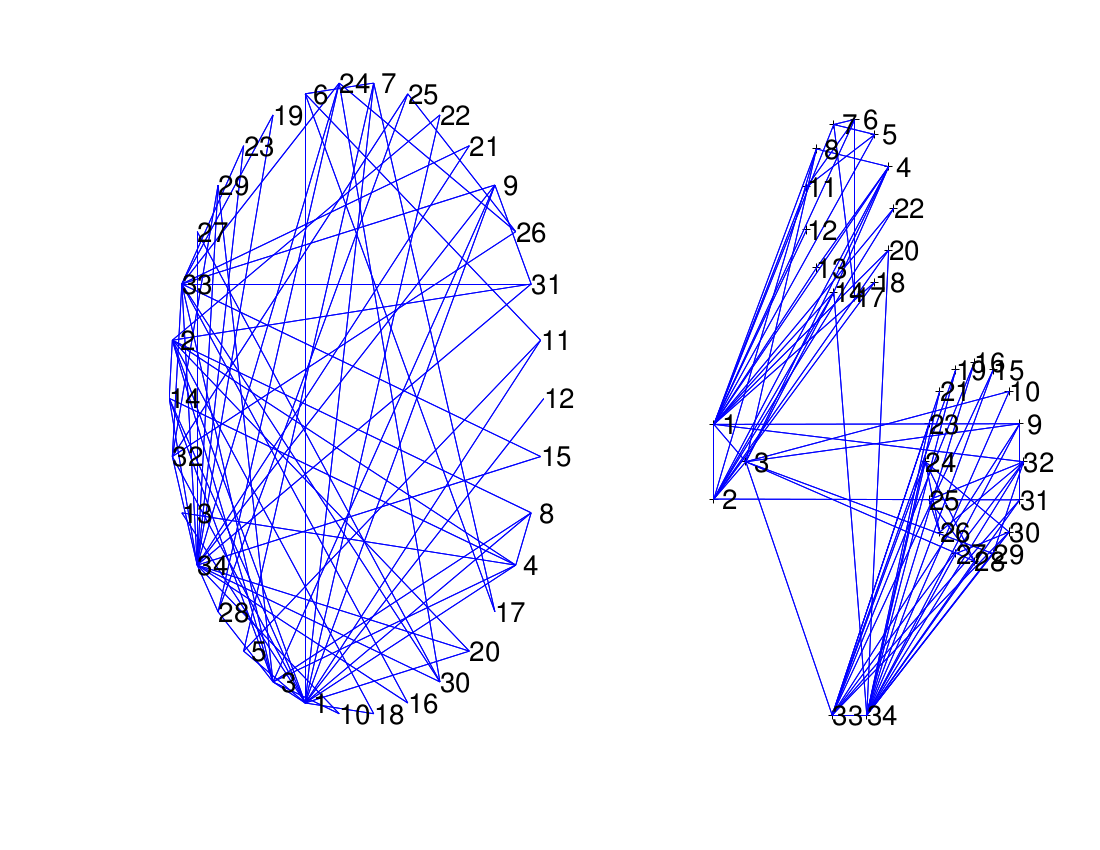
\epsfig{file = ../Figures/Karate-Graph.eps, clip=, width=7cm,
      height=9cm, angle=270, bbllx=75, bblly=485, bburx=535,
      bbury=765} \\ ~\\ ~\\
    Connexion probabilities \emphase{$\widehat{\pi}_{q\ell}$}:
    $$
    \left[ \begin{array}{rrrr}
        .99  &    .17 &    .07 &     \emphase{.74} \\
        -  &    1.00 &     \emphase{.53} &     .16 \\
        -  &    - &     .12 &      .00 \\
        -  &    - &      - &    .08 \\
      \end{array} \right]
    $$
    ~\\~\\
  \end{tabular}
\end{tabular}

% %$$
% \hspace{-1cm} 
% \begin{tabular}{lcccc}
%   %\vspace{-3cm}
%   \subsection{Structure} & Network & $Q$ & $\pi$ & Cluster. coef. \\
%   \hline
%   \begin{tabular}{p{2cm}} Random \\ (Erd�s-R�nyi) \end{tabular}
%   & \begin{tabular}{c} \epsfig{file = ../figures/FigNetworks-Erdos-Col.eps,
%       width=3cm, height=3cm, clip=, angle=270} 
%   \end{tabular}
%   & 1
%   &  $p$ & $p$ \\
%   \hline
%   \begin{tabular}{p{2cm}} Independent model (product connectivity) \end{tabular}
%   & \begin{tabular}{c} \epsfig{file = ../figures/FigNetworks-Indep-Col.eps,
%       width=3cm, clip=, angle=270}
%   \end{tabular}
%   & 2
%   & $\left( \begin{array}{cc} a^2 &ab\\ ab&b^2\\ \end{array}
%   \right)$
%   & $\displaystyle{\frac{(a^2+b^2)^2}{(a+b)^2}}$ \\
%   \hline
%   \begin{tabular}{p{2cm}} Stars \end{tabular}
%   & \begin{tabular}{c} 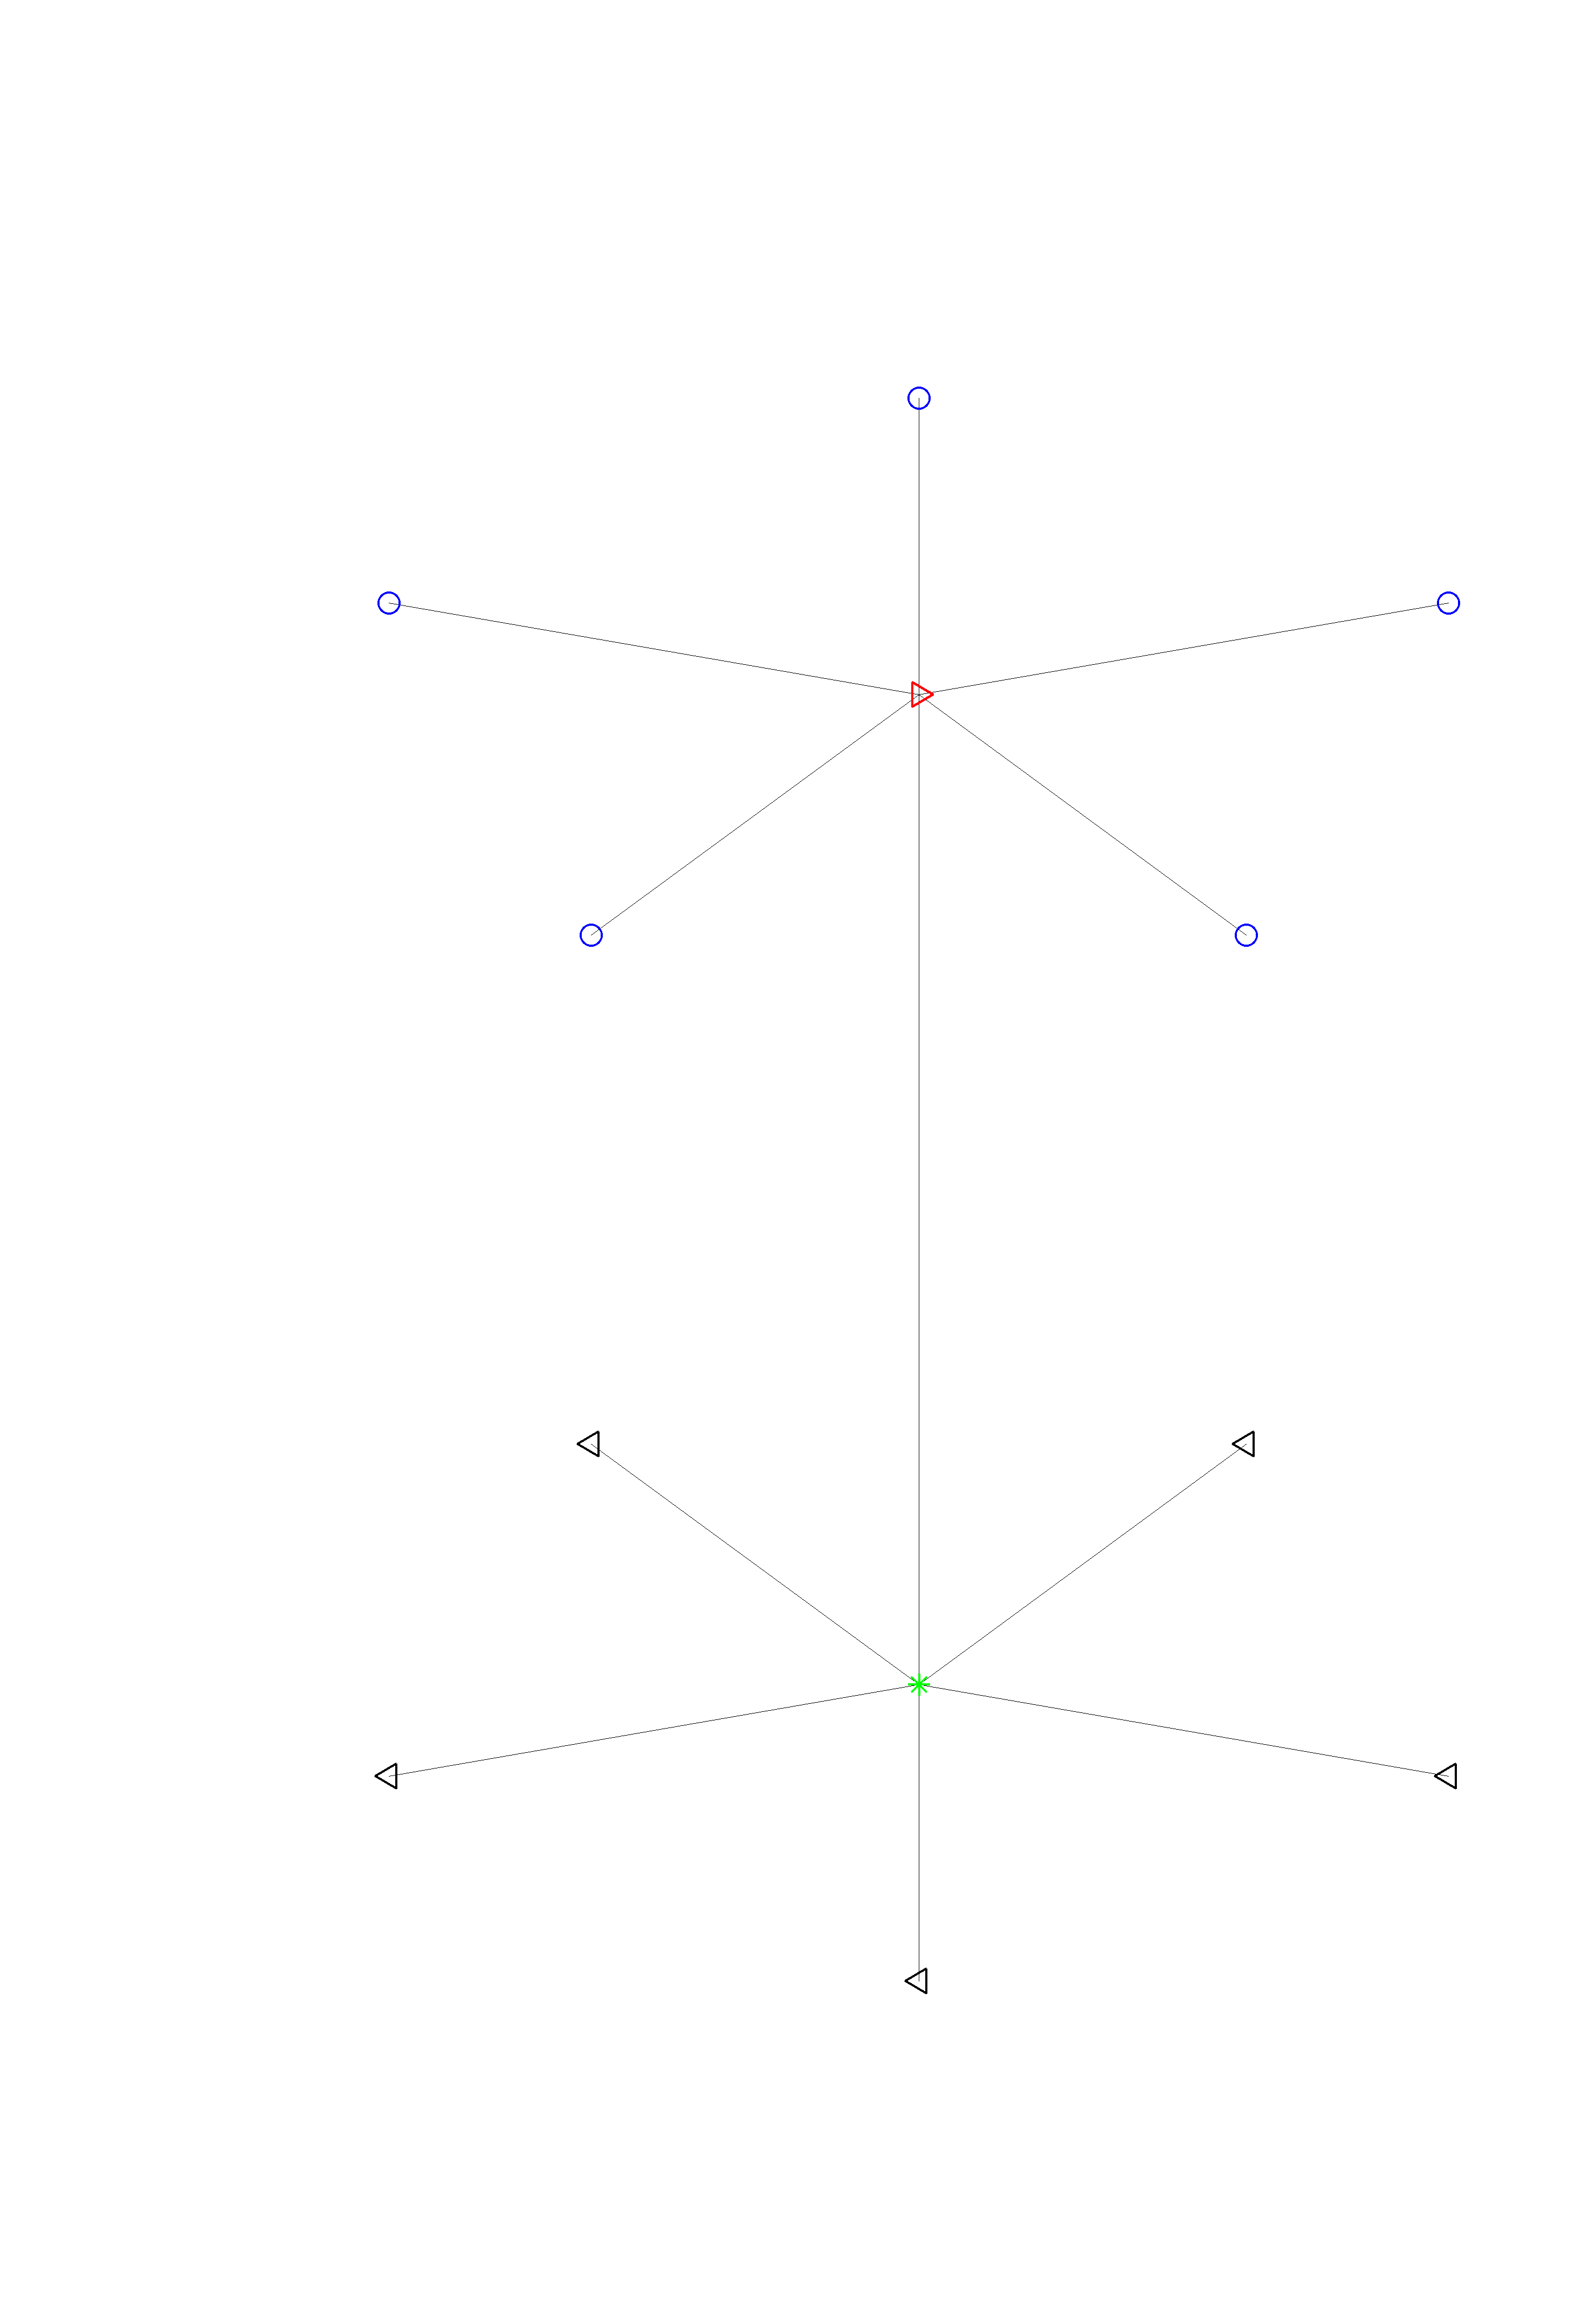
\epsfig{file = ../figures/FigNetworks-Star-Col.eps,
%       width=3cm, clip=, angle=270}
%   \end{tabular}
%   & 4
%   & $\left( \begin{array}{cccc} 0&1&0&0\\ 1&0&1&0\\0&1&0&1\\0&0&1&0\\
%     \end{array} \right)$
%   & 0 \\
%   \hline \begin{tabular}{p{2cm}} Clusters (affiliation networks)
%   \end{tabular} 
%   & \begin{tabular}{c} \epsfig{file = ../figures/FigNetworks-Clusters-Col.eps,
%       width=3cm, clip=, angle=270}
%   \end{tabular}
%   & 2
%   & $\left(\begin{array}{cc} 1&\varepsilon\\ \varepsilon&1\\
%     \end{array} \right)$ &
%   $\displaystyle{\frac{1+3\varepsilon^2}{(1+\varepsilon)^2}}$ \\ 
% \end{tabular} \\
% Similar to the block structure model (\refer{Novicki \& Snijders, 01})
% %$$
% % \paragraph{Scale free network model }
% %  (Barabasi \& Albert, 99) can also be expressed in terms of ERMG.

% %%%%%%%%%%%%%%%%%%%%%%%%%%%%%%%%%%%%%%%%%%%%%%%%%%%%%%%%%%%%%%%%%%%%%
% \newpage
% \subsection{Some probabilistic properties for binary graphs}
% %%%%%%%%%%%%%%%%%%%%%%%%%%%%%%%%%%%%%%%%%%%%%%%%%%%%%%%%%%%%%%%%%%%%%

% \paragraph{Conditional distribution of the degree:} Denoting $
% \pibar_q = \sum_{\ell} \alpha_{\ell} \pi_{q\ell}$, $\lambda_q = (n-1)
% \pibar_q$
% $$
% K_i \;|\; \{i \in q \} \sim \Bcal(n-1, \pibar_q) \approx
% \Pcal(\lambda_q).
% $$
% \bigskip\bigskip
% \paragraph{Marginal distribution of the degree:} we get a Poisson mixture
% $$
% K_i \sim \sum_q \Bcal(n-1, \pibar_q) \approx \sum_q \alpha_q \Pcal(\lambda_q).
% $$
% %%%%%%%%%%%%%%%%%%%%%%%%%%%%%%%%%%%%%%%%%%%%%%%%%%%%%%%%%%%%%%%%%%%%%
% %\newpage
% % \paragraph{Between-group connectivity.}
% % Let $A_{q\ell}$ denote the number of edges between groups $q$ and
% % $\ell$. Its expectation in the ERMG model is
% % $$
% % \Esp (A_{q\ell})  = \frac{n(n-1)}2 \alpha_q \alpha_{\ell} \pi_{q\ell}.
% % $$
% \paragraph{Clustering coefficient:}  
% $$
% c = \Pr\{\nabla \;|\; \Vsf\} = \Pr\{\nabla\} / \Pr\{\Vsf\} 
% = \frac{\sum_{q, \ell, m} \alpha_q \alpha_{\ell} \alpha_m \pi_{q\ell}
% \pi_{qm} \pi_{\ell m}}{\sum_{q, \ell, m} \alpha_q
%   \alpha_{\ell} \alpha_m \pi_{q\ell} \pi_{qm}}.
% $$

%%%%%%%%%%%%%%%%%%%%%%%%%%%%%%%%%%%%%%%%%%%%%%%%%%%%%%%%%%%%%%%%%%%%%
%%%%%%%%%%%%%%%%%%%%%%%%%%%%%%%%%%%%%%%%%%%%%%%%%%%%%%%%%%%%%%%%%%%%%
\newpage
\chapter{Variational inference}
%%%%%%%%%%%%%%%%%%%%%%%%%%%%%%%%%%%%%%%%%%%%%%%%%%%%%%%%%%%%%%%%%%%%%
%%%%%%%%%%%%%%%%%%%%%%%%%%%%%%%%%%%%%%%%%%%%%%%%%%%%%%%%%%%%%%%%%%%%%

%%%%%%%%%%%%%%%%%%%%%%%%%%%%%%%%%%%%%%%%%%%%%%%%%%%%%%%%%%%%%%%%%%%%%
\bigskip
\section{Maximum Likelihood Inference}
%%%%%%%%%%%%%%%%%%%%%%%%%%%%%%%%%%%%%%%%%%%%%%%%%%%%%%%%%%%%%%%%%%%%%

\paragraph{Likelihoods.} The log-likelihood of the complete dataset
($\Xbf, \Zbf$) is
\begin{eqnarray*}
  \log{\Pro(\Zbf,\Xbf; \alphabf, \thetabf)} & = & \log\Pro(\Zbf; \alphabf) +
    \log{\Pro(\Xbf | \Zbf; \thetabf)} \\
  & = & \sum_i \sum_q Z_{iq}\log{\alpha_q} + \sum_{i \neq j}
  \sum_{q,\ell} Z_{iq}Z_{j\ell}\log{f_{q\ell}(X_{ij})}.
\end{eqnarray*}
The log-likelihood of the observed dataset ($\Xbf$) is
$$
\log{\Pro(\Xbf; \alphabf, \thetabf)} = \sum_{\Zbf} \log{\Pro(\Zbf,\Xbf;
  \alphabf, \thetabf)}
$$
and cannot be evaluated since $\Zbf$ may take $Q^n$ different
values. \\

\paragraph{Most popular solution:} E-M algorithm.

%%%%%%%%%%%%%%%%%%%%%%%%%%%%%%%%%%%%%%%%%%%%%%%%%%%%%%%%%%%%%%%%%%%%%
\newpage
\paragraph{E-M algorithm.} To achieve the E-step, we need to calculate
the conditional distribution of the unobserved data given the observed
ones: $\log{\Pro(\Zbf|\Xbf)}$.

\paragraph{Due to intricate dependencies} this distribution is
\emphase{intractable}:
$$
\begin{tabular}{p{11cm}p{11cm}}
  \paragraph{Dependency graph} (oriented) & \paragraph{Moral graph}
  (parents are married) \\  
  \\
  Edge $X_{ij}$ only depends on its two parents $Z_1$ and $Z_2$
  &
  Conditional on the edges, labels $Z_i$'s all depend on each others \\
                                %\\
  \hspace{-1cm}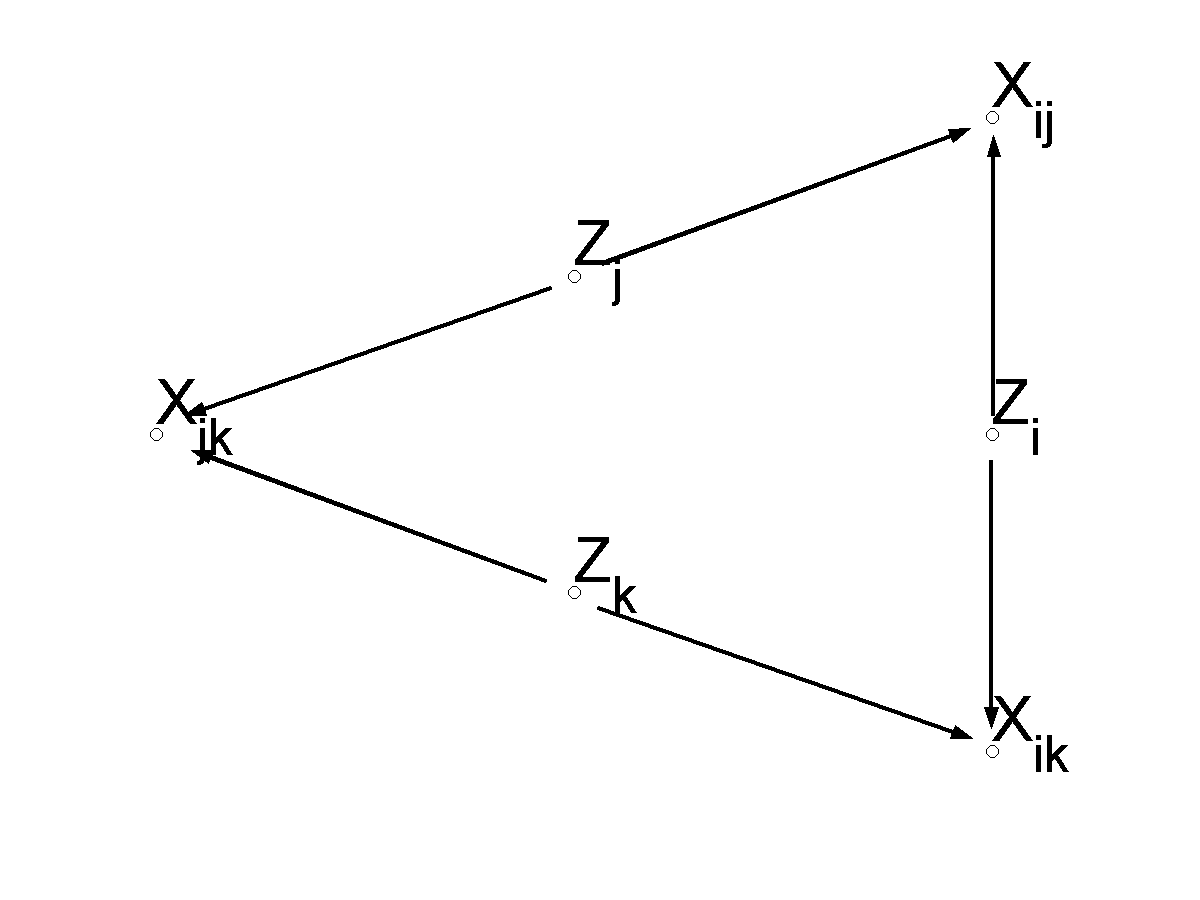
\epsfig{file = ../figures/FigNetworks-DepGraph.eps, clip=,
    angle=270, width=11cm}
  &
  \hspace{-1cm}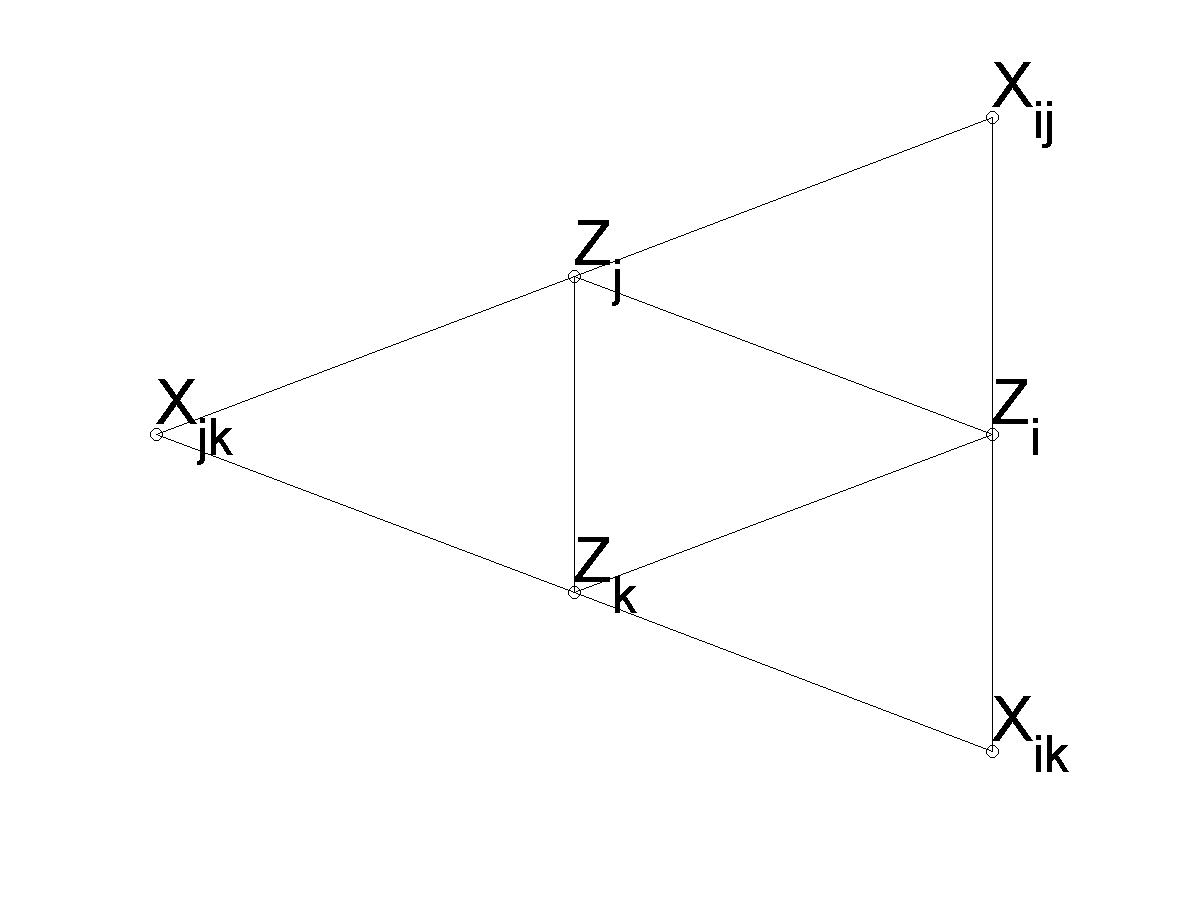
\epsfig{file = ../figures/FigNetworks-DepGraph-Moral.eps, clip=,
    angle=270, width=11cm} \\
  \multicolumn{2}{c}{\vspace{-0.5cm}$\Rightarrow$ All edges are
    actually \emphase{'neighbours'} (unlike in Bayesian networks).}
\end{tabular}
$$

%%%%%%%%%%%%%%%%%%%%%%%%%%%%%%%%%%%%%%%%%%%%%%%%%%%%%%%%%%%%%%%%%%%%%
\newpage
\section{Variational strategy}
%%%%%%%%%%%%%%%%%%%%%%%%%%%%%%%%%%%%%%%%%%%%%%%%%%%%%%%%%%%%%%%%%%%%%

\paragraph{Variational trick:} Maximise a \emphase{lower bound} of the
incomplete likelihood
$$
\Jcal(\RX,\alphabf, \thetabf) = \log{\Pro(\Xbf;\alphabf, \thetabf)} -
KL[\RX(\cdot),\Pro(\cdot|\Xbf;\alphabf, \thetabf)]
$$
where 
\begin{itemize}
\item \vspace{-0.5cm} $KL$ denotes the Kullback-Leibler divergence 
\item \vspace{-0.5cm} $\RX$ is some distribution for $\Zbf$.
\end{itemize}
Thanks to the definition of $KL$, we get for any $\RX$
(\refer{Jaakkola, 00})
\begin{eqnarray*}
  \Jcal(\RX,\alphabf, \thetabf) & = & \log{\Pro(\Xbf)} -
  \sum_{\Zbf} \log[\RX(\Zbf)] \RX(\Zbf) + \sum_{\Zbf}
  \log[P(\Zbf|\Xbf)] \RX(\Zbf) \\
  & = & \Hcal(\RX) + \sum_{\Zbf}
  \RX(\Zbf)\log{\Pro(\Xbf, \Zbf;\alphabf, \thetabf)}
\end{eqnarray*}
where $\Hcal(\RX)$ stands for the entropy of distribution $\RX$.

%%%%%%%%%%%%%%%%%%%%%%%%%%%%%%%%%%%%%%%%%%%%%%%%%%%%%%%%%%%%%%%%%%%%%
\newpage
\paragraph{Choice of $\RX$.} $\RX$ approximates the conditional
distribution $\Pro(\Zbf|\Xbf)$. We want it to be
\begin{itemize}
\item \vspace{-0.5cm} tractable (e.g. factorised):
  $$    
  \RX(\Zbf) = \prod_i h(\Zbf_i, \taubf_i)
  $$
  where $h(\cdot, \taubf)$ denotes the multinomial distribution;
\item \vspace{-0.5cm} as close to $\Pro(\Zbf|\Xbf)$ as possible:
  $$
  \widehat{\taubf} = \arg \min
  KL[\RX(\cdot),\Pro(\cdot|\Xbf;\alphabf, \thetabf)].
  $$
\end{itemize}
We get
$$
\Jcal(\RX,\alphabf, \thetabf) = - \sum_i \sum_q \tau_{iq} \log{\tau_{iq}} +
\sum_i \sum_q \tau_{iq} \log{\alpha_q} + \sum_{i \neq j} \sum_{q,\ell}
\tau_{iq} \tau_{j\ell} \log{f_{q\ell}(X_{ij})}.
$$
The $\tau_i$'s are interpreted as \emphase{approximate posterior
  probabilities $\Pro\{Z_i = q | \Xbf\}$};

%%%%%%%%%%%%%%%%%%%%%%%%%%%%%%%%%%%%%%%%%%%%%%%%%%%%%%%%%%%%%%%%%%%%%
\newpage
\subsection{Estimation algorithm}

The optimisation of $\Jcal(\RX,\alphabf, \thetabf)$ is achieved via two
alternative steps.

\paragraph{M-step:} Maximises $\Jcal(\RX,\alphabf, \thetabf)$ w.r.t. $\alphabf, \thetabf =
(\alphabf, \thetabf)$ given $\taubf$. We get
$$
\widehat{\alpha}_q = \frac1n \sum_i \tau_{iq}, \qquad
\widehat{\theta}_{q\ell} = \arg\underset{\theta_{q\ell}}{\max} \sum_{i
  \neq j} \tau_{iq}\tau_{j\ell}\log{f(X_{ij}; \theta_{q\ell})}.
$$

\paragraph{Pseudo E-step:} Finds the optimal $\taubf$ given
$(\alphabf, \thetabf)$. We end up with a \emphase{fix point relation}.
$$
\log \widehat{\tau}_{iq} = \mbox{cst} + \log \alpha_q + \sum_{j
  \neq i} \sum_{\ell} \widehat{\tau}_{j\ell} \log f(X_{ij};
\theta_{q\ell})
$$
which is equivalent to a \emphase{mean field} approximation.

\bigskip\bigskip
\paragraph{MixNet program:} For binary networks \\
\centerline{\url{stat.genopole.cnrs.fr/software/mixnet}}
(\refer{Miele \& al., ??})


%%%%%%%%%%%%%%%%%%%%%%%%%%%%%%%%%%%%%%%%%%%%%%%%%%%%%%%%%%%%%%%%%%%%%
\newpage
\section{Model selection}
%%%%%%%%%%%%%%%%%%%%%%%%%%%%%%%%%%%%%%%%%%%%%%%%%%%%%%%%%%%%%%%%%%%%%

\paragraph{Penalised likelihood.} Standard criteria, such as BIC or
AIC are based on the log-likelihood of observed data $\log
\Pro(\Xbf)$, so they can not be used here.

\paragraph{Integrated Classification Likelihood (ICL).} The ICL
criterion (\refer{Biernacki \& al., 00}) is an approximation of the
complete-data integrated log-likelihood:
$$
\log \Pro(\Xbf, \Zbf| m_Q) = \int \log \Pro(\Xbf, \Zbf |
\gammabf,m_Q) g(\gammabf|m_Q) d\gammabf,
$$
where $\log \Pro(\Xbf, \Zbf | \gammabf,m_Q)$ is the log-likelihood
of model $m_Q$ with $Q$ classes.

We get
$$
ICL(m_Q) = \underset{\gammabf}{\max} \log \Pro(\Xbf,
\widehat{\Zbf} |\gammabf, m_Q) - \frac{1}{2} \left\{ P_Q \log
  [n(n-1)] - (Q-1) \log(n) \right\}.
$$
where $P_Q$ denotes the number of parameters in $\thetabf$ and
$\widehat{\Zbf}$ can be replaced by $\widehat{\taubf}$ or by the
Maximum A posteriori (MAP) prediction of $\Zbf$.


%%%%%%%%%%%%%%%%%%%%%%%%%%%%%%%%%%%%%%%%%%%%%%%%%%%%%%%%%%%%%%%%%%%%%
%%%%%%%%%%%%%%%%%%%%%%%%%%%%%%%%%%%%%%%%%%%%%%%%%%%%%%%%%%%%%%%%%%%%%
\newpage
% \chapter{Applications to biological networks}
% %%%%%%%%%%%%%%%%%%%%%%%%%%%%%%%%%%%%%%%%%%%%%%%%%%%%%%%%%%%%%%%%%%%%%
% %%%%%%%%%%%%%%%%%%%%%%%%%%%%%%%%%%%%%%%%%%%%%%%%%%%%%%%%%%%%%%%%%%%%%

% %%%%%%%%%%%%%%%%%%%%%%%%%%%%%%%%%%%%%%%%%%%%%%%%%%%%%%%%%%%%%%%%%%%%%
% \bigskip
\section{Metabolic network of {\sl E. coli}}
%%%%%%%%%%%%%%%%%%%%%%%%%%%%%%%%%%%%%%%%%%%%%%%%%%%%%%%%%%%%%%%%%%%%%

\paragraph{Dataset.}
\begin{itemize}
\item \vspace{-0.5cm} The network is made of 605 reaction (nodes) and
  1782 edges (\refer{V Lacroix \& M.-F. Sagot, INRIA}).
\item \vspace{-0.5cm} Reactions $i$ and $j$ are connected if the
  compound of $i$ is the substrate of $j$.
\item \vspace{-0.5cm} Because most reactions are reversible, the
  network is not oriented.
\item \vspace{-0.5cm} The only information about edges is terms of
  presence/absence.
\end{itemize}
\paragraph{Results} 
\begin{itemize}
\item \vspace{-0.5cm} The ICL criterion applied to a mixture with
  Bernoulli edge values select $\widehat{Q} = 21$ classes.
    \item \vspace{-0.5cm} Groups 1 to 20 gather reactions involving
      all the \emphase{same compound} either as a substrate or as a
      product.
    \item \vspace{-0.5cm} A compound (chorismate, pyruvate,
      ATP,\emph{etc}) can be associated to each group.
\end{itemize}


%%%%%%%%%%%%%%%%%%%%%%%%%%%%%%%%%%%%%%%%%%%%%%%%%%%%%%%%%%%%%%%%%%%%%
\newpage
\paragraph{Dot-plot representation.} \\
\begin{tabular}{cc}
  \begin{tabular}{p{12cm}}
    \begin{itemize}
    \item Classes 1 and 16 constitute a \emphase{single clique}
      corresponding to a single compound (pyruvate),
    \item They are split into two classes because they
      \emphase{interact differently with classes 7} (CO2) and 10
      (AcetylCoA)
    \item Connectivity matrix (sample): 
      $$
      \begin{array}{c|cccc}
        q, \ell & 1 & 7 & 10 & 16 \\
        \hline
        1  & \textcolor{red}{1.0} & & & \\
        7  & \textcolor{green}{.11} & .65 & &  \\
        10 & \textcolor{green}{.43} & & .67 & \\
        16 & \textcolor{red}{1.0} & \textcolor{yellow}{.01} &
        \textcolor{yellow}{\epsilon} & \textcolor{red}{1.0}
      \end{array}
      $$
    \end{itemize}    
  \end{tabular}
  &
  \begin{tabular}{c}
      Adjacency matrix \\
      (zoom on the \emphase{first 20 classes}) \\
      \\
    \epsfig{file = ../Figures/Ecoli-Complet-ERMG-Ward-Q21_class3.ps,
     height=12cm, width=12cm, clip=, angle=90, bbllx=33, bblly=64,
    bburx=565, bbury=389} 
   \end{tabular}
\end{tabular}

% %%%%%%%%%%%%%%%%%%%%%%%%%%%%%%%%%%%%%%%%%%%%%%%%%%%%%%%%%%%%%%%%%%%%%
% \newpage
% \section{Gene regulations in {\sl A. Thaliana}}
% %%%%%%%%%%%%%%%%%%%%%%%%%%%%%%%%%%%%%%%%%%%%%%%%%%%%%%%%%%%%%%%%%%%%%

% \paragraph{Dataset.} \emphase{Partial correlations} between the expression
% levels of 800 genes in various conditions (\refer{Opgen-Rhein \&
%   Strimmer, 06}). \\
% ~\\
% \begin{tabular}{cc}
%   \hspace{-1cm}
%   \begin{tabular}{p{12cm}}
%     \paragraph{Dot-plot.} Dot size = absolute correlation, Color =
%     sign (\textred{$-$}, \textblue{$+$}). \\
%     ~\\
%     \paragraph{Results.} 
%     \begin{itemize}
%     \item \vspace{-0.5cm} Using a Gaussian model, we get $\widehat{Q}
%       = 7$ classes.
%     \item \vspace{-0.5cm} Groups are made of positively correlated
%       genes. 
%     \item \vspace{-0.5cm} Between group correlations are weaker than
%       within-group correlation and have different signs (see classes
%       3/4 with class 7).
%     \item \vspace{-0.5cm} Total computational time for $Q=1..15$
%       classes on a standard PC: 1h.
%     \end{itemize}
%   \end{tabular}
%   &
%   \begin{tabular}{c}
%     \hspace{-1cm}
%     \epsfig{file = ../Figures/GauHo_Q7_dotplot.eps, width=13cm,
%     height=13cm, clip=}
%   \end{tabular}
% \end{tabular}

%%%%%%%%%%%%%%%%%%%%%%%%%%%%%%%%%%%%%%%%%%%%%%%%%%%%%%%%%%%%%%%%%%%%%
\newpage
\section{Fungus - Tree interactions}
%%%%%%%%%%%%%%%%%%%%%%%%%%%%%%%%%%%%%%%%%%%%%%%%%%%%%%%%%%%%%%%%%%%%%

\paragraph{Dataset.} Interactions between 154 fungi and 51
trees European species. Fungus $f$ is connected to tree $t$ if it has
been collected on it (\refer{C. Vacher, INRA}).

\paragraph{Projected graphs.} For each species we define the projected
graph:
$$
\begin{array}{lrcl}
  \mbox{for trees} \quad & X_{tt'} & = & \mbox{Number of common
  fungi,} \\ 
\\
  \mbox{for fungi} \quad & X_{ff'} & = & \mbox{Number of common trees.}
\end{array}  
$$

\paragraph{Poisson model.} For both species, we assume that the
intensities have Poisson distributions: $X
\sim\Pcal(\lambda_{q\ell})$.

\paragraph{Number of classes.} The ICL criterion selects 
\begin{itemize}
\item \vspace{-0.5cm} 7 classes for trees
\item \vspace{-0.5cm} and 9 classes for fungi.
\end{itemize}



%%%%%%%%%%%%%%%%%%%%%%%%%%%%%%%%%%%%%%%%%%%%%%%%%%%%%%%%%%%%%%%%%%%%%
\newpage
\noindent
\begin{tabular}{cc}
  \begin{tabular}{p{14cm}}
    \subsection{Fungus network}
    \\ 
%     \epsfig{file = ../Figures/Fungus_Poiss_Q6_dotplot.eps,
%       width=12cm, height=12cm, clip=} \\
    \epsfig{file = ../Figures/Fungus_Poiss_Q9_dotplot.eps,
      width=13cm, height=13cm, clip=} \\
    \begin{itemize}
    \item \vspace{-0.5cm} A group of generalist fungi is detected.
    \item \vspace{-0.5cm} Others are more specific.
    \end{itemize}
  \end{tabular}
  &
  \begin{tabular}{p{8cm}}
    \subsection{Tree network}
    \\
%     \epsfig{file = ../Figures/Tree_Poiss_Q5_dotplot.eps,
%       width=8cm, height=8cm, clip=}
    \epsfig{file = ../Figures/Tree_Poiss_Q7_dotplot.eps,
      width=6cm, height=6cm, clip=}
    \\ 
    \begin{itemize}
    \item \vspace{-0.5cm} Trees are mainly clustered according to
      the number of fungi they host.
    \item \vspace{-0.5cm} Tree groups are less contrasted.
    \end{itemize}
    \\ \\ \\ \\ \\
  \end{tabular}
\end{tabular}

%%%%%%%%%%%%%%%%%%%%%%%%%%%%%%%%%%%%%%%%%%%%%%%%%%%%%%%%%%%%%%%%%%%%%
\newpage
\subsection{Cross-clustering}

%\bigskip
\noindent
\begin{tabular}{cc}
  \begin{tabular}{p{16cm}}
    The comparison of the two clusterings exhibits \emphase{specific
    correspondences} between groups of fungi (rows) and trees (columns). \\
    \\ \\
    \paragraph{(Partial) interpretation.} 
    \begin{itemize}
    \item Tree clusters are mainly related to their
      phyla, 
    \item \vspace{-0.5cm} whereas fungal groups mostly refer to their
      nutrition strategy... 
    \end{itemize}
    \\ \\
    \paragraph{Biclustering.} A direct clustering could be performed
    on the interaction matrix Fungi $\times$ Tree. The method
    proposed by \refer{Govaert \& Nadif (05)} also relies on a
    variational approach. \\ \\
  \end{tabular}
  &
  \begin{tabular}{p{10cm}}
%     \epsfig{file = ../Figures/CompCluster_QF6_QT5.eps,
%     width=7cm, height=15cm, clip=}
    \epsfig{file = ../Figures/CompCluster_QF9_QT7.eps,
    width=7cm, height=15cm, clip=}
  \end{tabular}
\end{tabular}


%%%%%%%%%%%%%%%%%%%%%%%%%%%%%%%%%%%%%%%%%%%%%%%%%%%%%%%%%%%%%%%%%%%%%
%%%%%%%%%%%%%%%%%%%%%%%%%%%%%%%%%%%%%%%%%%%%%%%%%%%%%%%%%%%%%%%%%%%%%
\newpage
\chapter{Motifs in interaction graphs}
%%%%%%%%%%%%%%%%%%%%%%%%%%%%%%%%%%%%%%%%%%%%%%%%%%%%%%%%%%%%%%%%%%%%%
%%%%%%%%%%%%%%%%%%%%%%%%%%%%%%%%%%%%%%%%%%%%%%%%%%%%%%%%%%%%%%%%%%%%%

%%%%%%%%%%%%%%%%%%%%%%%%%%%%%%%%%%%%%%%%%%%%%%%%%%%%%%%%%%%%%%%%%%%%%
\bigskip
\section{Topological motifs and permutations}
%%%%%%%%%%%%%%%%%%%%%%%%%%%%%%%%%%%%%%%%%%%%%%%%%%%%%%%%%%%%%%%%%%%%%

\paragraph{Definition.}  A motif $\mbf$ of size $k$ is a connected
sub-graph with $k$ vertices characterised by its adjacency matrix
(also denoted by $\mbf$):
$$
m_{uv} = \Ibb\{u \sim v\}.
$$
\hspace{-0.75cm}
\begin{tabular}{cc}
  \begin{tabular}{p{10cm}}
    \paragraph{Permutations.} For a given motif $\mbf$, we need to
    consider the set $\Rcal(\mbf)$ of its permutations
    (\emphase{automorphisms}). \\
    \\
    For example, the $\mathsf{V}$ motif may occure in 3 ways at a
    \emphase{fixed} position $\alpha = (i,j,k)$: \\
    \\
  \end{tabular}
  &
  \begin{tabular}{ccc}
    $\mbf$ &  $\mbf^{\prime}$ & $\mbf^{\prime \prime}$ \\
    & & \\
    $\left[ \begin{array}{ccc} 
        0 & 1 & 1 \\ . & 0 & 0 \\ . & . & 0 
      \end{array} \right]$  &
    $\left[ \begin{array}{ccc} 
        0 & 1 & 0 \\ . & 0 & 1 \\ . & . & 0 
      \end{array} \right]$ &
    $\left[ \begin{array}{ccc} 
        0 & 0 & 1 \\ . & 0 & 1 \\ . & . & 0 
      \end{array} \right] $ \\
    &&
    \\
    \epsfig{file=../Figures/version2.eps} & 
    \epsfig{file=../Figures/version3.eps} & 
    \epsfig{file=../Figures/version1.eps} 
  \end{tabular}
\end{tabular}

%%%%%%%%%%%%%%%%%%%%%%%%%%%%%%%%%%%%%%%%%%%%%%%%%%%%%%%%%%%%%%%%%%%%%
\newpage
\subsection{Count}

\paragraph{Position.} A ($k$-)position $\alpha$ is a set of $k$
different nodes taken is ascending order:
$$
\alpha = (i_1, ... i_k), \qquad i_1 < i_2 < ... < i_k.
$$
A graph of size $n$ contains \emphase{$\displaystyle{\binom{n}{k}}$
  positions}.

\paragraph{Occurrence.} $Y_{\alpha}(\mbf)$ is the \emphase{binary
  variable} indicating if $\mbf$ occurs at position $\alpha$:
$$
Y_{\alpha}(\mbf) 
= \Ibb\{\mbf \text{ occurs at } \alpha\}
=\prod_{1 \leq u < v \leq k} (X_{i_ui_v})^{m_{uv}}.
$$

\paragraph{Count.} The total number of occurrences of $\mbf$ in the
graph is the sum over \emphase{all positions} and \emphase{all
  permutations} of the binary variables $Y_{\alpha}(\mbf)$:
$$
N(\mbf) = \sum_{\alpha} \sum_{\mbf' \in \Rcal(\mbf)} Y_{\alpha}(\mbf').
$$

%%%%%%%%%%%%%%%%%%%%%%%%%%%%%%%%%%%%%%%%%%%%%%%%%%%%%%%%%%%%%%%%%%%%%
\newpage
\section{Exact Moments of the Count}
%%%%%%%%%%%%%%%%%%%%%%%%%%%%%%%%%%%%%%%%%%%%%%%%%%%%%%%%%%%%%%%%%%%%%

%%%%%%%%%%%%%%%%%%%%%%%%%%%%%%%%%%%%%%%%%%%%%%%%%%%%%%%%%%%%%%%%%%%%%
\bigskip\bigskip
\subsection{Two hypotheses} 
%%%%%%%%%%%%%%%%%%%%%%%%%%%%%%%%%%%%%%%%%%%%%%%%%%%%%%%%%%%%%%%%%%%%%

\paragraph{(H1) Stationarity:}
$$ 
\Dcal(X_{i_1j_1}, \ldots, X_{i_{\ell}j_{\ell}}) = \Dcal
(X_{i'_1j'_1}, \ldots, X_{i'_{\ell}j'_{\ell}}). 
$$
\bigskip
\paragraph{(H2) Independence of disjoint occurrences:}
$$
Y_\alpha(\mbf) \perp Y_\beta(\mbf) \quad \text{ if } \quad \alpha
\cap \beta =\emptyset.  
$$

%%%%%%%%%%%%%%%%%%%%%%%%%%%%%%%%%%%%%%%%%%%%%%%%%%%%%%%%%%%%%%%%%%%%%
\bigskip%\bigskip
\subsection{Occurrence probability} 
%%%%%%%%%%%%%%%%%%%%%%%%%%%%%%%%%%%%%%%%%%%%%%%%%%%%%%%%%%%%%%%%%%%%%

Thanks to (H1), the probability for $\mbf$ to occur at position
$\alpha$ does not depend on $\alpha$. For symmetry reasons, it is the
same for all the permutations of $\mbf$:
$$
\forall \alpha, \forall \mbf' \in \Rcal(\mbf), \qquad
\Pr\{Y_{\alpha}(\mbf') = 1\} = \Pr\{Y_{\alpha}(\mbf) = 1\} = \mum.
$$

%%%%%%%%%%%%%%%%%%%%%%%%%%%%%%%%%%%%%%%%%%%%%%%%%%%%%%%%%%%%%%%%%%%%%
\newpage
\subsection{Calculating the occurrence probability}

The occurrence probability \emphase{$\mum$} is the central quantity of
this approach. It depends on the random graph model.

\paragraph{Erd�s-Renyi:}
$$
\mum = \prod_{1 \leq u<v \leq k} \pi^{m_{uv}} = \pi^{m_{++}/2}.
$$

\paragraph{Expected Degree Distribution (EDD):} Suppose that $K$ has a
distribution proportional to the empirical degree distribution and
denote ${m_{u+}}$ the number of edges of node $u$ in motif $\mbf$,
$$
\mum \propto \prod_{u=1}^k \Esp\left(K^{m_{u+}} \right).
$$

\paragraph{Mixture model:}
$$
\mum   =   \sum_{c_1=1}^{Q} \hdots \sum_{c_k=1}^{Q}
\alpha_{c_1}\hdots \alpha_{c_k} \prod_{1 \leq u<v \leq k}
\pi_{c_u,c_v}^{m_{uv}}.
$$

%%%%%%%%%%%%%%%%%%%%%%%%%%%%%%%%%%%%%%%%%%%%%%%%%%%%%%%%%%%%%%%%%%%%%
\newpage
\subsection{Exact Moments}

%%%%%%%%%%%%%%%%%%%%%%%%%%%%%%%%%%%%%%%%%%%%%%%%%%%%%%%%%%%%%%%%%%%%%
\paragraph{Mean:} 
The calculation of the expected count is straightforward:
$$
\Esp N(\mbf) = \sum_{\alpha} \sum_{\mbf' \in \Rcal(\mbf)}
\Esp Y_{\alpha}(\mbf') = \binom{n}{k} |\Rcal(\mbf)| \mum.
$$

%%%%%%%%%%%%%%%%%%%%%%%%%%%%%%%%%%%%%%%%%%%%%%%%%%%%%%%%%%%%%%%%%%%%%
\paragraph{Variance:} 
The variance is obtained via the calculation of $\Esp N(\mbf)^2$. The
squared count is 
\begin{eqnarray*}
  N^2(\mbf) & = & \sum_{\alpha, \beta \in I_k}
  \sum_{\mbf^\prime, \mbf''\in \mathcal{R}(\mbf)}
  Y_{\alpha}(\mbf')Y_{\beta}(\mbf'') \\
  & = & \sum_{s=0}^k \sum_{|\alpha \cap \beta| = s}
  \sum_{\mbf', \mbf'' \in \Rcal(\mbf)} Y_{\alpha \cup \beta}(\mbf'
\Omegas \mbf'')
\end{eqnarray*}
where $\Omegas$ is the \emphase{overlapping operator} with $s$
common nodes and $\mbf' \Omegas \mbf''$ is the \emphase{super-motif}
made of two overlapping occurrences of $\mbf'$ and $\mbf''$.


%%%%%%%%%%%%%%%%%%%%%%%%%%%%%%%%%%%%%%%%%%%%%%%%%%%%%%%%%%%%%%%%%%%%%
\newpage
\hspace{-2.2cm}
\begin{tabular}{cc}
  \begin{tabular}{p{12cm}}
    \paragraph{Super-motifs} are made of overlapping
    occurrences of equivalent versions of $\mbf$. \\
    \\
    \paragraph{Enumeration.} The adjacency matrices of all
    super-motifs can be listed \emphase{automatically}. \\
    The algorithm consist in the systematic exploration of all $\mbf'
    \Omegas \mbf''=$ 
    $$
    \left(\begin{array}{c|c|c}
        \mbf'_{11} & \mbf'_{12} & \Obf \\
        \hline
        \mbf'_{21} & \max(\mbf'_{22}, \mbf''_{11}) &  \mbf''_{12} \\
        \hline
        \Obf  & \mbf''_{21} &  \mbf''_{22} \\
      \end{array} \right).
    $$
    \\ \\
    \paragraph{Right:} All $\mbf' \Omegas \mbf''$ with $s=3$
    for the 4 spike star motif: \\
    \centerline{\begin{tabular}{cc}
        \begin{tabular}{c} $\mbf = $ \end{tabular} & 
        \begin{tabular}{c} \hspace{-2cm}     
          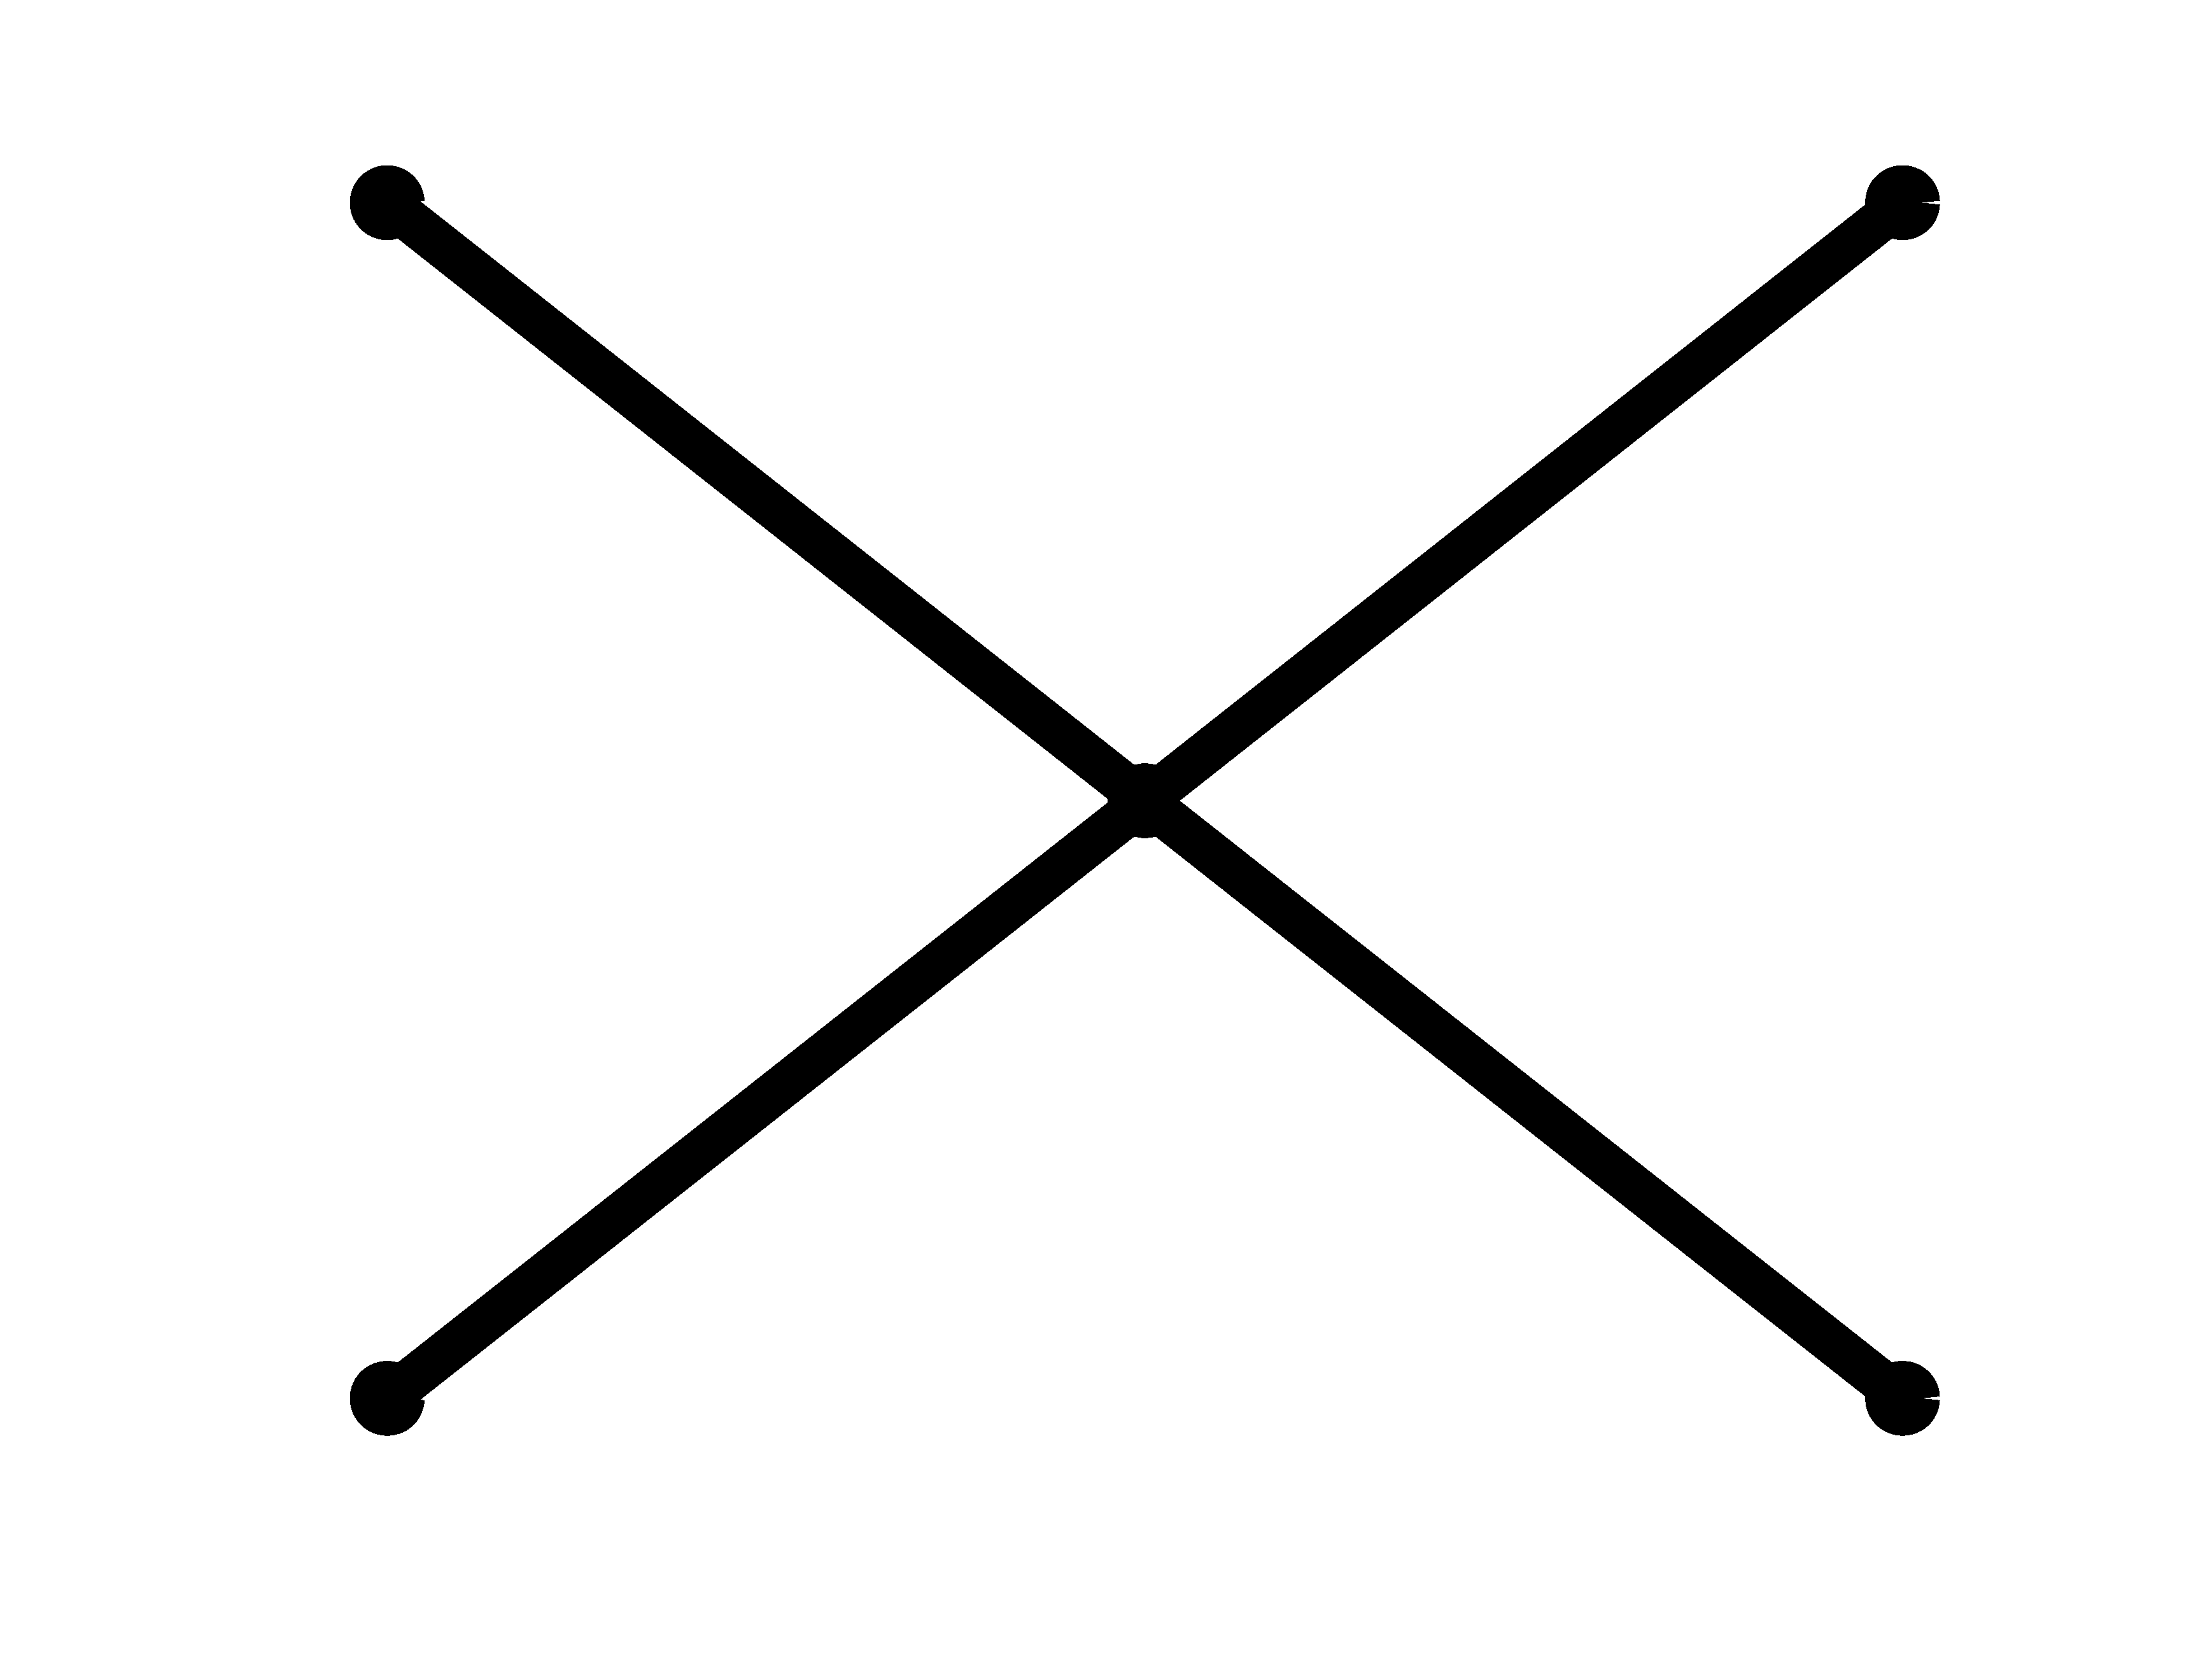
\epsfig{file = ../Figures/Motif-Star4.eps, clip=, 
            width=1cm, height=1cm}
        \end{tabular}   
      \end{tabular}  } 
  \end{tabular}
  &
  \begin{tabular}{c}
    \hspace{-1cm}
    \epsfig{file= ../../Motifs/FIGURES/MotifStar4-Recouv3.eps,
      clip=, width=13cm, height=17cm}
  \end{tabular}
\end{tabular}

%\paragraph{Variance.} The formula of the variance follows:
  
%%%%%%%%%%%%%%%%%%%%%%%%%%%%%%%%%%%%%%%%%%%%%%%%%%%%%%%%%%%%%%%%%%%%%
%%%%%%%%%%%%%%%%%%%%%%%%%%%%%%%%%%%%%%%%%%%%%%%%%%%%%%%%%%%%%%%%%%%%%
\newpage
\chapter{Approximate distribution for the count}
%%%%%%%%%%%%%%%%%%%%%%%%%%%%%%%%%%%%%%%%%%%%%%%%%%%%%%%%%%%%%%%%%%%%%
%%%%%%%%%%%%%%%%%%%%%%%%%%%%%%%%%%%%%%%%%%%%%%%%%%%%%%%%%%%%%%%%%%%%%

%%%%%%%%%%%%%%%%%%%%%%%%%%%%%%%%%%%%%%%%%%%%%%%%%%%%%%%%%%%%%%%%%%%%%
\subsection{Motif count distribution: State of the art}

\paragraph{Asymptotic approximations (Gaussian, Poisson, Compound
  Poisson)}. Many papers about the asymptotic distribution of the
  count $\Nm$. 
\begin{itemize}
\item Most of the times, only \emphase{simple models} (Erd�s-R�nyi) or
  \emphase{simple motifs} (triangle) are considered (\refer{Janson,
    00}).
\item The underlying hypotheses are very \emphase{restrictive} and
  depend on the structure of the motif itself.
\end{itemize}

\bigskip\bigskip
\paragraph{Standard approach in biological applications.}
When analysing motifs in biological networks, the most common strategy
is based on simulations, empirical moments and/or empirical
distribution (\refer{Shen-Orr \& al, 02}; \refer{Milo \& al., 02, 04}).

%%%%%%%%%%%%%%%%%%%%%%%%%%%%%%%%%%%%%%%%%%%%%%%%%%%%%%%%%%%%%%%%%%%%%
\newpage
\subsection{Compound Poisson approximation}

\paragraph{Compound Poisson distribution.} All network motifs can overlap (and
constitute super-motifs) so they tend to \emphase{occur in clumps}.
The compound Poisson distribution states that 
\begin{itemize}
\item \vspace{-0.5cm} the number of clumps $C(\mbf)$ has a Poisson
  distribution $\Pcal(\lambda)$;
\item \vspace{-0.5cm} the clump sizes $V_1, ..., V_{C(\mbf)}$ are i.i.d.
\end{itemize}
The count $\Nm$ is the sum of the clump sizes: $\Nm = \sum_c V_c$.

\bigskip\bigskip
\paragraph{Geometric Poisson approximation.} Analogy with
\emphase{sequence motifs} (\refer{R. \& al., 03}) suggests that the
clump size has a geometric distribution, $\Gcal(1-a)$ where $a$ is the
\emphase{overlapping probability of the motif}.

Parameters $\lambda$ and $a$ are related two the first two moments:
$$
a = \frac{\Var\Nm - \Esp\Nm}{\Var\Nm + \Esp\Nm}, \qquad
\lambda = (1-a) \Esp\Nm.
$$

%%%%%%%%%%%%%%%%%%%%%%%%%%%%%%%%%%%%%%%%%%%%%%%%%%%%%%%%%%%%%%%%%%%%%
\newpage
\section{Simulation study}
%%%%%%%%%%%%%%%%%%%%%%%%%%%%%%%%%%%%%%%%%%%%%%%%%%%%%%%%%%%%%%%%%%%%%

% \subsection{Simulation design}

% \paragraph{Aim:} Compare the Gaussian, Poisson and Geometric-Poisson
% approximations for the motif count distribution.

% \hspace{-2.2cm}
% \begin{tabular}{cc}
%   \begin{tabular}{p{12cm}}
%     \paragraph{Random graph model:} Mixture model with 2 groups.
%     \\ \\
%     \paragraph{4 motifs:}  \\
%     %$$
%     \begin{tabular}{cccc}
%       $\mathsf{V}$ & triangle & 4-star & square \\
% %       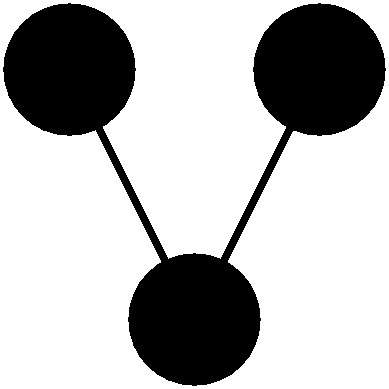
\includegraphics[height=1cm]{../figures/Vmotif.eps} & 
% %       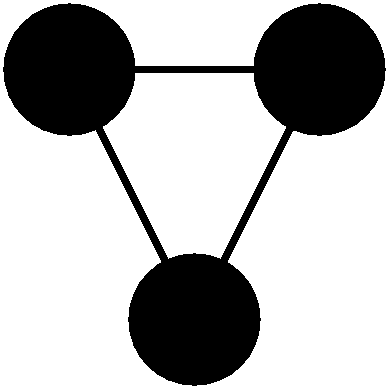
\includegraphics[height=1cm]{../figures/trianglemotif.eps} & 
% %       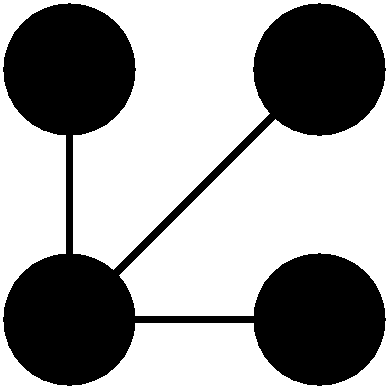
\includegraphics[height=1cm]{../figures/starmotif.eps}  & 
% %       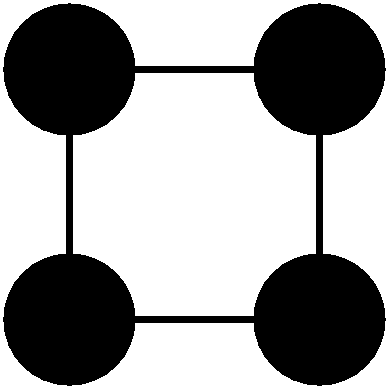
\includegraphics[height=1cm]{../figures/squaremotif.eps}\\
%       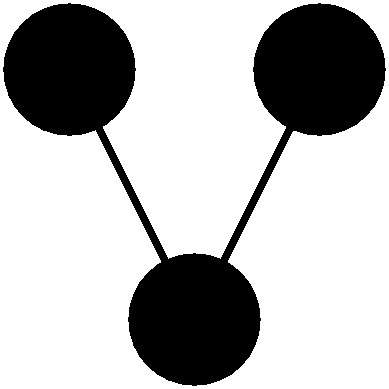
\epsfig{file = ../figures/Vmotif.eps, width=2cm, clip=} & 
%       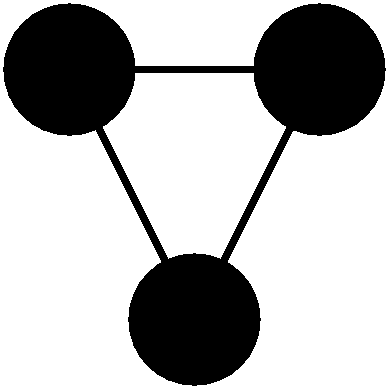
\epsfig{file = ../figures/trianglemotif.eps, width=2cm, clip=} & 
%       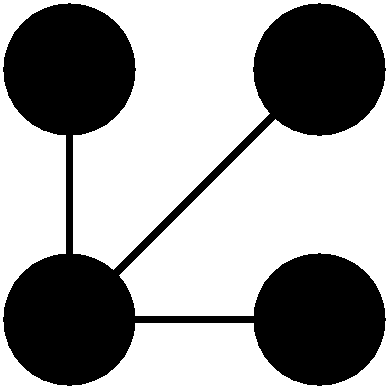
\epsfig{file = ../figures/starmotif.eps, width=2cm, clip=}  & 
%       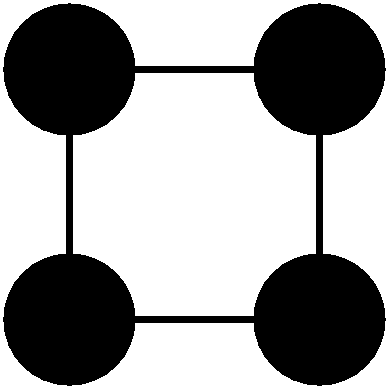
\epsfig{file = ../figures/squaremotif.eps, width=2cm, clip=}
%     \end{tabular}
%     %$$
%   \end{tabular}
%   &
%   \begin{tabular}{p{12cm}}
%     \paragraph{Simulation design:}
%     \begin{itemize}
%     \item \vspace{-0.5cm} number of vertices $n=20,200$
%     \item \vspace{-0.5cm} mean connectivity $\bar{\pi}=1/n,2/n$ 
%     \item \vspace{-0.5cm} within/between group connectivity
%       $\gamma=0.1,0.5,0.9$ 
%     \item \vspace{-0.5cm} proportion of the groups $\alpha=0.1,0.9$
%     \end{itemize}
%   \end{tabular}
% \end{tabular}

% \paragraph{Expected frequency:}
% We cover a large range for $\Esp N(\mbf)$ (from 0.07 to 1075.5).

% \hspace{-1.75cm}
% \begin{tabular}{cl}
%   \paragraph{Criterion:} & $D =$ total variation distance, \\
%   & $\widehat{F} = $ actual level of the 99\% theoretical quantile
%   (should be 1\%).
% \end{tabular}

% %%%%%%%%%%%%%%%%%%%%%%%%%%%%%%%%%%%%%%%%%%%%%%%%%%%%%%%%%%%%%%%%%%%%%
% \newpage
% \subsection{Expectedly frequent motif count distribution}

% \hspace{-2.2cm}
% \begin{tabular}{cc}
%   \multicolumn{2}{c}{Gaussian ($G = $ \textcolor{red}{--}), Poisson (--) and
%     Geometric-Poisson ($GP = $ \textcolor{green}{--})} \\
%     Histogram & PP-plot \\
%     \epsfig{file = ../figures/hist_200_0.005_0.5_0.1_V.eps,
%     width=12cm, clip=} 
%     &
%     \epsfig{file = ../figures/PPPlot_200_0.005_0.5_0.1_V.eps,
%     width=12cm, clip=}  
% \end{tabular} \\
% \hspace*{-1cm}
% \begin{tabular}{cc}
%   {\small simulation parameters} &  motif $\Vsf$ \\
%   {\small
%     \begin{tabular}{c|c|c|c}
%       $n$ & $\overline{\pi}$ & $\alpha$ (\%)& $\gamma$ (\%)\\ \hline
%       200     & 0.5   & 10    & 10   \\
%       200     & 0.5   & 10    & 90   \\
%       200     & 0.5   & 50    & 10   \\
%       200     & 0.5   & 50    & 50   \\
%       200     & 0.5   & 50    & 90  \\
%     \end{tabular} 
%     } 
%   &
%   {\small
%     \begin{tabular}{c|c|c|c|c|c|c|c}
%       $\Esp$ & $\mathbb{V}$ & $\lambda$ & $\frac{1}{1-a}$  & $D_G$ & $D_{GP}$ &
%       $\hat{F}_G$ & \emphase{$\hat{F}_{GP}$} \\ \hline
%       159.5   & 2034.0        & 23.1 & 6.66   & 20.4 & 19.7 & 2.5 & \emphase{1.6} \\
%       104.9   & 590.5         & 31.6 & 3.33   & 15.2 & 14 & 1.9 & \emphase{1.2}\\
%       98.5    & 484.0         & 33.3 & 2.27   & 13.1 & 12.6 & 1.1 & \emphase{0.7}\\
%       98.5    & 484.0         & 33.2 & 2.27   & 14.3 & 13.2 & 1.6 & \emphase{1.1}\\
%       98.5    & 488.4         & 33.1 & 2.27   & 14.5 & 14.8 & 2.5 & \emphase{0.9}\\
%     \end{tabular}
%     }
%   \\
% \end{tabular}

% %%%%%%%%%%%%%%%%%%%%%%%%%%%%%%%%%%%%%%%%%%%%%%%%%%%%%%%%%%%%%%%%%%%%%
% \newpage
% \subsection{Expectedly rare motif count distribution}

% \hspace{-2.2cm}
% \begin{tabular}{cc}
%   \multicolumn{2}{c}{Gaussian ($G = $ \textcolor{red}{--}), Poisson (--) and
%     Geometric-Poisson ($GP = $ \textcolor{green}{--})} \\
%     Histogram & PP-plot \\
%     \epsfig{file = ../figures/hist_200_0.01_0.1_0.1_C.eps, 
%     width=12cm, clip=} 
%     &
%     \epsfig{file = ../figures/PPPlot_200_0.01_0.1_0.1_C.eps,
%     width=12cm, clip=}  
% \end{tabular} \\
% \hspace*{-1cm}
% \begin{tabular}{cc}
%   {\small simulation parameters} &  motif $\square$ \\
%   {\small
%     \begin{tabular}{c|c|c|c}
%       $n$ & $\overline{\pi}$ & $\alpha$ (\%)& $\gamma$ (\%)\\ \hline
%       200     & 0.5   & 10    & 10   \\
%       200     & 0.5   & 10    & 90   \\
%       200     & 0.5   & 50    & 10   \\
%       200     & 0.5   & 50    & 50   \\
%       200     & 0.5   & 50    & 90  \\
%     \end{tabular} 
%     } 
%   &
%   {\small
%     \begin{tabular}{c|c|c|c|c|c|c|c}
%       $\Esp$ & $\mathbb{V}$ & $\lambda$ & $\frac{1}{1-a}$  & $D_G$ & $D_{GP}$ &
%       $\hat{F}_G$ & \emphase{$\hat{F}_{GP}$} \\ \hline
%       7.31&21.72&3.68& 2 &11.8&5.4&3.2&\emphase{0.9}\\
%       2.57&3.42&2.21 & 1.16 &9.3&2.7&3.6&\emphase{0.5}\\
%       2.74&3.69&2.33 & 1.17 &12.3&3.6&4.7&\emphase{1.2}\\
%       1.94&2.40&1.74 & 1.11  &11.3&2.0&3.2&\emphase{1.6}\\
%       2.74&3.72&2.32 & 1.17 &10.8&4.5&3.7&\emphase{0.7}\\
%     \end{tabular}
%     }
%   \\
% \end{tabular}

% %%%%%%%%%%%%%%%%%%%%%%%%%%%%%%%%%%%%%%%%%%%%%%%%%%%%%%%%%%%%%%%%%%%%%
% \newpage
% \subsection{Conclusions for the simulation study}

\begin{itemize}
% \item Correct analytical expressions for $\Esp N$ and
%   $\Var N$ (simulations not shown).
\item Bad fit of the Poisson approximation.
\item \emphase{Geometric-Poisson outperforms Gaussian} in all cases,
  especially for ``rare'' motifs, in terms of both
  \begin{itemize}
  \item total variation distance and
  \item quantile precision.
  \end{itemize}
\item \emphase{Underestimation of the 99\% quantile}
  with the Gaussian approximation, \\
  {\bf{$\rightarrow$}} false positive results.
\item \emphase{High total variation distance} for both
  approximations in some cases, especially for frequent and highly
  self overlapping motifs.
\item The clumps size distribution is probably \emphase{not geometric}
  $\ldots$
\end{itemize}

%%%%%%%%%%%%%%%%%%%%%%%%%%%%%%%%%%%%%%%%%%%%%%%%%%%%%%%%%%%%%%%%%%%%%
\newpage
\section{Application to the {\it H. pylori} PPI network}
%%%%%%%%%%%%%%%%%%%%%%%%%%%%%%%%%%%%%%%%%%%%%%%%%%%%%%%%%%%%%%%%%%%%%

Protein-protein interaction network: 706 proteins (nodes) and 1420
interactions (edges).

\hspace{-2cm}
\begin{tabular}{cc}
  \begin{tabular}{p{12cm}}
    \subsection{Fit of the mixture model} \\
    \begin{itemize}
    \item \vspace{-0.5cm} The mixture was fitted to the network and
      \emphase{4 groups} of connectivity were selected using a model
      selection criterion (ICL).
    \item \vspace{-0.5cm} Goodness-of-fit for the degree distribution
      assessed by PP-plot (right).
    \end{itemize}
  \end{tabular}
  &
  \begin{tabular}{c}
    \epsfig{file = ../figures/hist-deg-HPylo.eps, width=10cm, clip=}   
  \end{tabular}
\end{tabular}

%%%%%%%%%%%%%%%%%%%%%%%%%%%%%%%%%%%%%%%%%%%%%%%%%%%%%%%%%%%%%%%%%%%%%
\newpage
\subsection{Significance of motifs of size 3 and 4}

2 motifs appear to be unexpectedly frequent.
$$
\begin{tabular}{crrrrrr}
 Motif & $N_{\obs}(\mbf)$ & $\Esp_{\ERMG}(N)$ & $\sigma_{\ERMG}(N)$ &
 $\lambda$ & $1/(1-a)$ & $p$-value  \\

 \hline
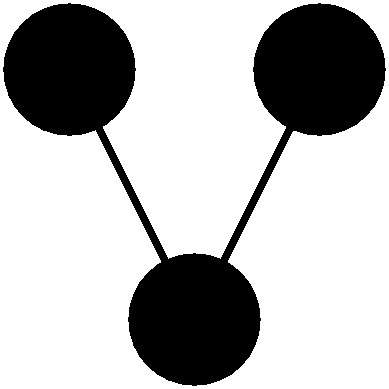
\epsfig{file = ../figures/Vmotif.eps, width=1cm, clip=} & 14\,113 & 13\,118 & 2\,599 & 25.5 & 514.9 & 3.36$\,10^{-1}$ \\
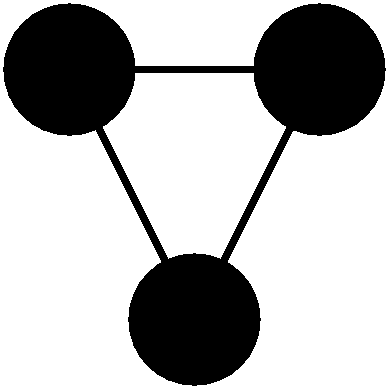
\epsfig{file = ../figures/trianglemotif.eps, width=1cm, clip=} & 75 & 64.4 & 20 & 10.4 & 6.2 & 2.87$\,10^{-1}$ \\
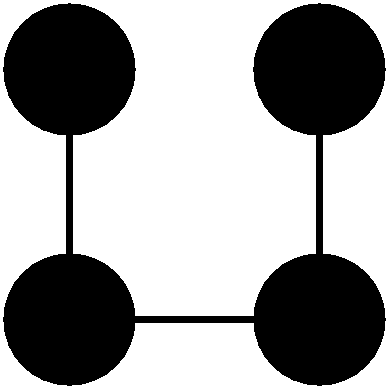
\epsfig{file = ../figures/chainmotif.eps, width=1cm, clip=} & 98\,697 & 90\,059 & 26\,064 & 11.9 & 7\,543.2 & 3.46$\,10^{-1}$ \\
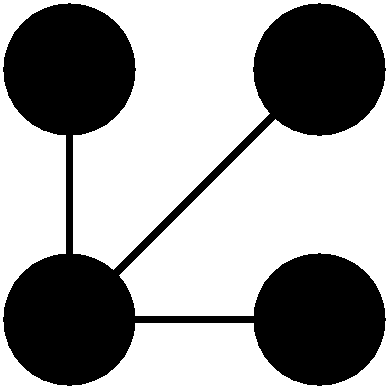
\epsfig{file = ../figures/starmotif.eps, width=1cm, clip=} & 112\,490 & 89\,372 & 26\,423 & 11.4 & 7\,812.0 & 1.85$\,10^{-1}$ \\
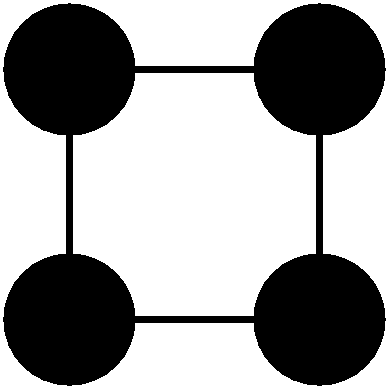
\epsfig{file = ../figures/squaremotif.eps, width=1cm, clip=} & 1\,058 & 492 & 202 & 5.9 & 82.9 & \emphase{9.34$\,10^{-3}$} \\
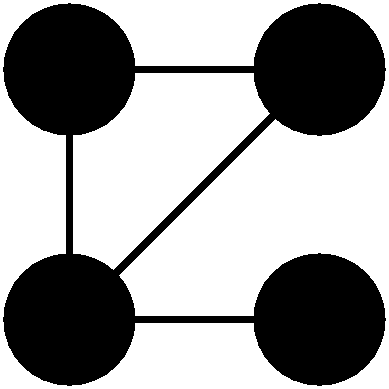
\epsfig{file = ../figures/whisker.eps, width=1cm, clip=} & 3\,535 & 2\,756 & 1\,087 & 6.4 & 428.7 & 2.22$\,10^{-1}$ \\
\epsfig{file = ../figures/halfclique.eps, width=1cm, clip=} & 79 &
 33.2 & 19.5 & 2.9 & 11.5 & \emphase{2.56$\,10^{-2}$} \\
\epsfig{file = ../figures/clique.eps, width=1cm, clip=} & 0 & 0.165 & 0.432 & 0.1 & 1.1 & 1.00 \\
\end{tabular}
$$
\paragraph{Mean clump size.} $\Esp V = 1/(1-a)$.

%%%%%%%%%%%%%%%%%%%%%%%%%%%%%%%%%%%%%%%%%%%%%%%%%%%%%%%%%%%%%%%%%%%%%
\newpage
\subsection{Comparison with the Mfinder software}

\bigskip
\centerline{{\tt Mfinder: www.weizmann.ac.il/mcb/UriAlon/}}

\bigskip
\hspace{-2cm}
\begin{tabular}{ll}
  \begin{tabular}{p{10cm}}
    \subsection{Motifs of size 3 and 4:} \\
    \\
    \emphase{All motifs are significantly} over- or
    under-represented...\\
    \\
    All empirical $p$-values are equal either to 0 or 1 (not shown). \\
    \\
    Simular results with 1000 simulated graphs. \\
    \\
  \end{tabular}
  &
  \hspace{-1.5cm}
  \begin{tabular}{c}
    {\small
      \begin{tabular}{c|r|rr|rrr|c} 
        Motif & $N_{\text{obs}}$ &
        $\overline{N}_{100}$&$\overline{\sigma }_{100}$&Z-score &
        $\Ncal$ $$p$$-value \\
        \hline
        \epsfig{file = ../figures/Vmotif.eps, width=1cm, clip=}     &  13\,888 
        & {13\,648} & {51.8} & \emphase{4.63} & {1.82\,10${^{-6}}$}    \\
        \epsfig{file = ../figures/trianglemotif.eps, width=1cm, clip=}   &  75    
        & {155}   & {17.3} & \emphase{-4.63}& {1.82\,10${^{-6}}$}     \\
        \epsfig{file = ../figures/chainmotif.eps, width=1cm, clip=} &  87\,869 
        & {112\,532} & {1\,957} & \emphase{-12.60}& {1.05\,10${^{-36}}$}  \\
        \epsfig{file = ../figures/starmotif.eps, width=1cm, clip=}  &  109\,113
        & {103\,186} & {1\,084} & \emphase{5.47}& {2.27\,10${^{-8}}$}     \\
        \epsfig{file = ../figures/squaremotif.eps, width=1cm, clip=}&  979   
        & {796} & {64.7} & \emphase{2.84}& {2.25\,10${^{-3}}$}    \\
        \epsfig{file = ../figures/whisker.eps, width=1cm, clip=}      &  3\,219  
        & {8\,734} & {945} & \emphase{-5.84}& {2.61\,10${^{-9}}$}   \\
        \epsfig{file = ../figures/halfclique.eps, width=1cm, clip=} &  79    
        & {273} & {66.7}& \emphase{-2.90}& {1.85\,10${^{-3}}$}    \\
        \epsfig{file = ../figures/clique.eps, width=1cm, clip=}     &  0     
        & {6.2} & {3.7} & \emphase{-1.70}& {4.45\,10${^{-2}}$}       
      \end{tabular}
      }
  \end{tabular}
\end{tabular}

\bigskip
\paragraph{Direct comparison can not be made} since MFinder considers
'induced' motifs, i.e. pure 'V', pure square, etc.

% %%%%%%%%%%%%%%%%%%%%%%%%%%%%%%%%%%%%%%%%%%%%%%%%%%%%%%%%%%%%%%%%%%%%%
% \newpage
% \subsection{Questions about the Mfinder 'model'}
% \begin{itemize}
% \item \vspace{-0.5cm} \paragraph{The model is not explicit.} The edge
%   swapping algorithm aims at sampling (uniformly?) among all the
%   graphs with \emphase{exactly the same degree sequence}. The
%   independence of the simulations relies on a \emphase{large number of
%     swaps}.
% \item \vspace{-0.5cm} \paragraph{The edge swapping algorithm} does not
%   really affect \emphase{strong network structure}: the number of
%   hubs, 'V''s and stars remains constant. \\
%   (The variability of the 'V' count is only due to the variability of
%   number of triangles.)
% \item \vspace{-0.5cm} \paragraph{What is the fit} of a model declaring
%   that \emphase{all motifs} are significant?
% \end{itemize}

% \subsection{Alternative}
% \begin{itemize}
% \item \vspace{-0.5cm} \paragraph{The Mfinder model} is stationary, but
%   distinct occurrences are not independent.
% \item \vspace{-0.5cm} \paragraph{EDD} may be a good alternative:
%   \begin{itemize}
%   \item \vspace{-0.5cm} It is similar to the 'Mfinder' model, but
%     \emphase{more flexible};
%   \item the moments can be calculated
%     exactly under EDD, which \emphase{avoids a costly resampling step}.
%   \end{itemize}
% \end{itemize}
 
% %%%%%%%%%%%%%%%%%%%%%%%%%%%%%%%%%%%%%%%%%%%%%%%%%%%%%%%%%%%%%%%%%%%%%
% \bigskip\bigskip
% \subsection{New simulations}

% \paragraph{Exact degree fitting (EDF) model.} We sampled without
% replacement in the observed degree distribution $\widehat{F}$ (similar
% to edge swapping in MFinder).

% \paragraph{Motif.} For each simulated graphs we counted the number of
% occurrences of each motif (with our definition). 

% %%%%%%%%%%%%%%%%%%%%%%%%%%%%%%%%%%%%%%%%%%%%%%%%%%%%%%%%%%%%%%%%%%%%%
% \newpage
% \subsection{Results for {\sl H. pylori.} PPI network}
% $$
% \begin{tabular}{cc}
%   \begin{tabular}{p{9cm}}
%     \paragraph{Comparison Mixture / EDF.}\\
%     \\ \\
%     Degree distribution fitting is a very strong constraint. \\
%     \\ \\
%     The number of occurrences of \emphase{star-like motifs} ('V', hubs,
%     {\it etc.})  is \emphase{completely fixed} in the EDF model.
%     \\ \\
%   \end{tabular}
%   &
%   \begin{tabular}{c}
%     \hspace{-1cm}
%     \begin{tabular}{c|rr|rr}
%       & \multicolumn{2}{c|}{$\overline{N}$} & \multicolumn{2}{c}{$\sigma(N)$} \\
%       Motif & Mixture & EDF & Mixture & EDF \\
%       \hline
%       \epsfig{file = ../figures/Vmotif.eps, width=1cm, clip=}         & 13 118  & 14 113  & 2 599   & \emphase{0} \\
%       \epsfig{file = ../figures/trianglemotif.eps, width=1cm, clip=}       & 64      & 53      & 20      & 8       \\
%       \epsfig{file = ../figures/chainmotif.eps, width=1cm, clip=}     & 90 059  & 84 106  & 26 064  & 3 283   \\
%       \epsfig{file = ../figures/starmotif.eps, width=1cm, clip=}      & 89 372  & 112 490 & 26 423  & \emphase{0} \\
%       \epsfig{file = ../figures/squaremotif.eps, width=1cm, clip=}    & 492     & 285     & 202     & 27      \\
%       \epsfig{file = ../figures/whisker.eps, width=1cm, clip=}          & 2 756   & 2 412   & 1 087   & 447     \\
%       \epsfig{file = ../figures/halfclique.eps, width=1cm, clip=}     & 33      & 22      & 20      & 10      \\
%       \epsfig{file = ../figures/clique.eps, width=1cm, clip=}        & 0.2     &  0.1     &  0.4     &   0.3     \\
%     \end{tabular}
%   \end{tabular}
% \end{tabular}
% $$

%%%%%%%%%%%%%%%%%%%%%%%%%%%%%%%%%%%%%%%%%%%%%%%%%%%%%%%%%%%%%%%%%%%%%
%%%%%%%%%%%%%%%%%%%%%%%%%%%%%%%%%%%%%%%%%%%%%%%%%%%%%%%%%%%%%%%%%%%%%
\newpage
\chapter{Discussion \& Work in progress}
%%%%%%%%%%%%%%%%%%%%%%%%%%%%%%%%%%%%%%%%%%%%%%%%%%%%%%%%%%%%%%%%%%%%%
%%%%%%%%%%%%%%%%%%%%%%%%%%%%%%%%%%%%%%%%%%%%%%%%%%%%%%%%%%%%%%%%%%%%%

%%%%%%%%%%%%%%%%%%%%%%%%%%%%%%%%%%%%%%%%%%%%%%%%%%%%%%%%%%%%%%%%%%%%%
\subsection{Inference for heterogeneous valued graphs}

\begin{itemize}
\item \vspace{-0.5cm} Mixture models constitutes a natural way to
  describe heterogeneity in a network.
\item \vspace{-0.5cm} The variational approach is a general and
  efficient alternative to MCMC algorithms.
\end{itemize}

%%%%%%%%%%%%%%%%%%%%%%%%%%%%%%%%%%%%%%%%%%%%%%%%%%%%%%%%%%%%%%%%%%%%%
\subsection{Applications of the mixture model}

\begin{itemize}
\item \vspace{-0.5cm} 'Realistic' heterogeneous networks can be
  simulated according to mixture models with given parameters.
\item \vspace{-0.5cm} Once fitted to a given network, the mixture
  model allows to detect unexpetedly frequent motifs in biological
  (binary) networks.
% \item \vspace{-0.5cm} The \emphase{Expected Degree Distribution (EDD)}
%   model (\refer{Park \& Newman, 03}, \refer{Chung \& Lu, 02}) is
%   another special case of heterogeneous binary network:
%   \begin{itemize} 
%   \item For each node $i$, draw its \emphase{expected degree $D_i$} in
%     the empirical degree distribution $F$ of a given network.
%     %: $\{D_i\} \mbox{ i.i.d. }  \sim F$.
%   \item For each couple of nodes $(i, j)$, the edge \emphase{$i \sim
%       j$ exists with probability $D_i D_j/K$}.
%     %: $(X_{ij} |D_i, D_j) \sim \Bcal(D_i D_j /K)$.
%   \end{itemize}
\end{itemize}

%%%%%%%%%%%%%%%%%%%%%%%%%%%%%%%%%%%%%%%%%%%%%%%%%%%%%%%%%%%%%%%%%%%%%
\subsection{Extension}
\begin{itemize}
\item \vspace{-0.5cm} The variational approach does not provide any
  measure of the precision of the estimates. \\
  $\rightarrow$ A variational Bayes (\refer{Beal \& Ghahramani, 03})
  approach would provide the (approximate) posterior distribution of
  the parameters.
\end{itemize}


%%%%%%%%%%%%%%%%%%%%%%%%%%%%%%%%%%%%%%%%%%%%%%%%%%%%%%%%%%%%%%%%%%%%%
\newpage
\subsection{Exceptional motifs}
%%%%%%%%%%%%%%%%%%%%%%%%%%%%%%%%%%%%%%%%%%%%%%%%%%%%%%%%%%%%%%%%%%%%%

\begin{itemize}
\item \vspace{-0.5cm} We propose a general method to \emphase{assess
    the exceptionality of network motifs}.
\item \vspace{-0.5cm} The formula of the moments are valid for a
  \emphase{large class} of random graphs.
\item \vspace{-0.5cm} The \emphase{geometric Poisson approximation
    performs well} (better than Gaussian and Poisson) on simulated
  data.
\end{itemize}

%%%%%%%%%%%%%%%%%%%%%%%%%%%%%%%%%%%%%%%%%%%%%%%%%%%%%%%%%%%%%%%%%%%%%
\subsection{In progress}

\begin{itemize}
\item \vspace{-0.5cm} Insights about the \emphase{distribution of the
    clump size} (other than geometric) would improve the compound
  Poisson approximation. 
\item \vspace{-0.5cm} \emphase{Model averaging} (\refer{Hoeting \&
    al., 99}) avoids to choose one number of clusters in a mixture.
\item \vspace{-0.5cm} \emphase{A colored motif} is a connected subset
  set of colored. Such motifs can describe protein complexes, the
  proteins being classified into functions.  \\
  \centerline{$\Rightarrow$ How to assess their exceptionality?
    (\refer{Schbath \& al., ??})}
\item \vspace{-0.5cm} \emphase{What is a relevant random graph model}
  for motif detection. \\
  \centerline{$\Rightarrow$ What properties should it satisfy?}
\end{itemize}

% %%%%%%%%%%%%%%%%%%%%%%%%%%%%%%%%%%%%%%%%%%%%%%%%%%%%%%%%%%%%%%%%%%%%
% \newpage
% \section{Mixture model as a null model for heterogeneous networks}

% \noindent
% \begin{tabular}{cc}
%   \begin{tabular}{p{15cm}}
%     \paragraph{Looking for over-represented motifs in {\sl E. coli}
%     transcriptional network.} \\
%     \\
%     \paragraph{Strategy proposed by \refer{\sl Shen-Orr \& al, 02}.} 
%     \begin{enumerate}
%     \item Count the number of occurrences $N_{\obs}(\mbf)$;
%     \item Resample a \textblue{large number of random networks}
%       similar to {\sl E.coli}'s one (using the edge swapping
%       algorithm);
%     \item Estimate $\Esp \Nm$ and $\Var \Nm$;
%     \item Calculate a $Z$-score: 
%       $Z = (N_{\obs}(\mbf) - \Esp \Nm)/ \sqrt{\Var \Nm}$;
%     \item \textblue{Derive a $p$-value} implicitly based on a Gaussian
%       approximation. 
%     \end{enumerate}
%   \end{tabular}
%   &
%   \begin{tabular}{c}
%     \epsfig{file=../FIGURES/RegulationMotifs.ps, bbllx=82, bblly=89,
%     bburx=289, bbury=600, clip=, height=16cm}
%   \end{tabular}
% \end{tabular}

% %%%%%%%%%%%%%%%%%%%%%%%%%%%%%%%%%%%%%%%%%%%%%%%%%%%%%%%%%%%%%%%%%%%%
% \newpage
% \subsection{Direct computation using heterogenous models}

% \noindent \hspace{-1cm}
% \begin{tabular}{cc}
%   \begin{tabular}{p{11cm}}
%     \paragraph{Exact moments.} For several heterogeneous models
%     (mixture, EDD), we can get the exact formula for the mean $\Esp N$
%     and variance $\Var N$ of the count (\refer{Picard \& al., 07}). \\
%     \\ \\
%     \paragraph{Distribution.} Based on theoretical results (Erd�s)
%     and an analogy with sequence motifs, we fit a \emphase{compound
%     Poisson} distribution to derive a $p$-value. \\ \\
%   \end{tabular}
%   &
%   \begin{tabular}{p{10cm}}
%     {\small \hspace{-1cm}
%     \begin{tabular}{crrrr}
%       Motif & $N_{\obs}(\mbf)$ & $\lambda$ & $\displaystyle{\frac1{(1-a)}}$ & $p$-value  \\
%       \hline
%       \epsfig{file = ../figures/Vmotif.eps, width=1cm, clip=} & 14\,113 & 25.5 & 514.9 & 3.36$\,10^{-1}$ \\
%       \epsfig{file = ../figures/trianglemotif.eps, width=1cm, clip=} & 75 & 10.4 & 6.2 & 2.87$\,10^{-1}$ \\
%       \epsfig{file = ../figures/chainmotif.eps, width=1cm, clip=} & 98\,697 & 11.9 & 7\,543.2 & 3.46$\,10^{-1}$ \\
%       \epsfig{file = ../figures/starmotif.eps, width=1cm, clip=} & 112\,490 & 11.4 & 7\,812.0 & 1.85$\,10^{-1}$ \\
%       \epsfig{file = ../figures/squaremotif.eps, width=1cm, clip=} & 1\,058 & 5.9 & 82.9 & \emphase{9.34$\,10^{-3}$} \\
%       \epsfig{file = ../figures/whisker.eps, width=1cm, clip=} & 3\,535 & 6.4 & 428.7 & 2.22$\,10^{-1}$ \\
%       \epsfig{file = ../figures/halfclique.eps, width=1cm, clip=} & 79 & 2.9 & 11.5 & \emphase{2.56$\,10^{-2}$} \\
%       \epsfig{file = ../figures/clique.eps, width=1cm, clip=} & 0 & 0.1 & 1.1 & 1.00 \\
%     \end{tabular}
%     }
%   \end{tabular}
% \end{tabular}

% \paragraph{Results for \emphase{E. coli}'s network.} 2 motifs
% appear to be unexpectedly frequent. \\
% \\
% According to the permutation-based strategy, all of them are
% significantly over-represented!


% %%%%%%%%%%%%%%%%%%%%%%%%%%%%%%%%%%%%%%%%%%%%%%%%%%%%%%%%%%%%%%%%%%%%
% \newpage
% \section{Variational Bayes approach}

% \refer{Beal \& Ghahramani (2003)} propose a 
% \begin{itemize}
% \item \vspace{-0.5cm} variational
% \item \vspace{-0.5cm} Bayes 
% \item \vspace{-0.5cm} E-M algorithm 
% \end{itemize}
% to deal with for incomplete data models in the exponential family context.

% %%%%%%%%%%%%%%%%%%%%%%%%%%%%%%%%%%%%%%%%%%%%%%%%%%%%%%%%%%%%%%%%%%%%%
% \bigskip\bigskip
% \subsection{3-step approximation}

% \bigskip\bigskip
% \paragraph{1 - Variational approximation.} 
% Denoting $\thetabf$ the set of parameters, for any distribution $Q$,
% we have
% $$
% \log P(\Xbf) 
% \geq
% \int Q(\Zbf, \thetabf) \log
%     \frac{P(\Xbf, \Zbf, \thetabf)}{Q(\Zbf, \thetabf)} \dd \Zbf \dd
%     \thetabf 
% =: \Fcal(\Xbf, Q).
% $$

% %%%%%%%%%%%%%%%%%%%%%%%%%%%%%%%%%%%%%%%%%%%%%%%%%%%%%%%%%%%%%%%%%%%%
% \newpage
% \paragraph{2 - Optimal approximate distribution.}
% If we choose $Q = \Qt \QZ$, the optimal $\QZ$ and $\Qt$ must satisfy
% \begin{eqnarray*}
%   \QZ(\Zbf) & \propto & \exp \int \Qt(\thetabf) \log
%   P(\Xbf, \Zbf, \thetabf) \dd \thetabf, \\
%   \Qt(\thetabf) & \propto & \exp \int \QZ(\Zbf) \log P(\Xbf, \Zbf,
%   \thetabf) \dd \Zbf.
% \end{eqnarray*}
% This can be viewed as a \emphase{mean field} approximation.

% \bigskip\bigskip
% \paragraph{3 - Exponential family.}
% Suppose the complete likelihood belongs to the exponential family is and that parameter prior is conjugate
% \begin{eqnarray*}
%   P(\Xbf, \Zbf | \thetabf) &= & f(\Xbf, \Zbf) g(\thetabf)
%   \exp\{\phibf(\thetabf)' \ubf(\Xbf, \Zbf)\}, \\
%   \\
%   P(\thetabf |\eta, \nubf) & = & h(\eta, \nubf) g(\thetabf)^{\eta} \exp
%   \{\phibf(\thetabf)' \nubf\}.
% \end{eqnarray*}

% %%%%%%%%%%%%%%%%%%%%%%%%%%%%%%%%%%%%%%%%%%%%%%%%%%%%%%%%%%%%%%%%%%%%
% \newpage
% \subsection{Variational Bayes E-M algorithm}

% The optimal approximate conditional distribution $\Qt$ and $\QZ$ must
% satisfy
% $$
% \begin{array}{rclcrcl}
%   \Qt(\thetabf) & \propto & g(\thetabf)^{\tilde{\eta}}
%   \exp\{\phibf(\thetabf)' \tilde{\nubf}\},  
%   & \quad & \tilde{\eta} & = & \eta + 1, \\
%   \\
%   \overline{\ubf}(\Xbf) & = & \int \QZ(\thetabf) \ubf(\Xbf, \Zbf) \dd \Zbf;
%   & \quad & \tilde{\nubf} & = & \nubf + \overline{\ubf}(\Xbf, \Zbf),
%   \\ 
%   \\
%   \QZ(\Zbf) & \propto & f(\Xbf, \Zbf) \exp \left\{\overline{\phibf}'
%     \ubf(\Xbf, \Zbf) \right\}, 
%   & \quad &  \overline{\phibf} & = & \int \Qt(\thetabf) \phibf(\thetabf)
%   \dd \thetabf. 
% \end{array}
% $$

% \bigskip\bigskip
% \paragraph{Iterative algorithm.}
% The variational Bayes E-M algorithm consists in alternative updates of
% $\Qt$ ('E-step') and $\QZ$ ('M-step'):
% $$
% \begin{array}{rrcl}
%   \text{\bf E-step:} &   \Qt^{t+1}(\thetabf) & = & h(\tilde{\eta},
%   \tilde{\nubf}^t) g(\thetabf)^{\tilde{\eta}}
%   \exp\{[\phibf(\thetabf)]' \tilde{\nubf}^t\}; \\ 
%   \\
%   \text{\bf M-step:} &   \QZ^{t+1}(\Zbf) & \propto & f(\Xbf, \Zbf)
%   \exp \left\{\left[\overline{\phibf}^{t+1}\right]' \ubf(\Xbf, \Zbf)
%   \right\}. 
% \end{array}
% $$

% %%%%%%%%%%%%%%%%%%%%%%%%%%%%%%%%%%%%%%%%%%%%%%%%%%%%%%%%%%%%%%%%%%%%
% \newpage
% \subsection{Application to mixture in networks?}

% \paragraph{Interest.}
% \begin{itemize}
% \item \vspace{-0.5cm} Get \emphase{'confidence intervals'} for the
%   parameter;
% \item \vspace{-0.5cm} Still avoids costly MCMC algorithms.
% \end{itemize}

% \bigskip\bigskip
% \paragraph{Problems.}
% \begin{itemize}
% \item \vspace{-0.5cm} The approximate distribution $\QZ$ still needs
%   to be restricted (e.g. $\QZ = \prod_i \QZi$);
% \item \vspace{-0.5cm} Initialisation (same as E-M);
% \item \vspace{-0.5cm} Uniqueness of the fix point?
% \item \vspace{-0.5cm} The \emphase{intrinsic identifiability problem}
%   of mixture models...
% \end{itemize}


%%%%%%%%%%%%%%%%%%%%%%%%%%%%%%%%%%%%%%%%%%%%%%%%%%%%%%%%%%%%%%%%%%%%%%%%
\newpage
\subsection{Articles}
\begin{itemize}
\item S. Robin F. Picard, J.-J. Daudin. A mixture model for random
  graphs. Stat. Comput., 18(2):173--83, Jun 2008.
\item F. Picard, J.-J. Daudin, M. Koskas, S. Schbath, and S. Robin
  Assessing the exceptionality of network motifs,. J. Comp. Biol.,
  15(1):1--20, 2008
\item C. Matias, S. Schbath, E. Birmel�, J.-J. Daudin, and S. Robin.
  Networks motifs : mean and variance for the count. RevStat, pages
  31--51, 2006. \url{www.ine.pt/revstat/pdf/rs060102.pdf}.
\end{itemize}

%%%%%%%%%%%%%%%%%%%%%%%%%%%%%%%%%%%%%%%%%%%%%%%%%%%%%%%%%%%%%%%%%%%%%%%%
\subsection{Research report}
\begin{itemize}
\item M. Mariadassou and S. Robin. Uncovering latent structure in
  valued graphs: a variational approach.  SSB Report \#10, October 2007: \\
  \url{genome.jouy.inra.fr/ssb/preprint/SSB-RR-10.valued-graphs.pdf}.
\end{itemize}


%%%%%%%%%%%%%%%%%%%%%%%%%%%%%%%%%%%%%%%%%%%%%%%%%%%%%%%%%%%%%%%%%%%%
\newpage
\chapter{Additional slides}

%%%%%%%%%%%%%%%%%%%%%%%%%%%%%%%%%%%%%%%%%%%%%%%%%%%%%%%%%%%%%%%%%%%%
\newpage
\subsection{'Inhomogeneous' random graphs}

\paragraph{General definition for binary graphs.} (\refer{Bollob\'as \ al., 07})
\begin{itemize}
\item \vspace{-0.5cm} $n$ nodes $(i = 1 \dots n$)
\item \vspace{-0.5cm} $n(n-1)/2$ possible edges: $X_{ij} = \Ibb\{ i \sim j\}$
\item \vspace{-0.5cm} Each $i$ is characterised by a \emphase{latent
    variable} $Z_i$ sampled in some space $\Zcal$ with distribution
  $\alpha$:
  $$
  \{Z_i\}_i \mbox{ i.i.d.}, \qquad Z_i \sim \alpha
  $$
\item \vspace{-0.5cm} Edge $(i, j)$ is present with probability
  $\pi(Z_i, Z_j)$, where $\pi$ is a \emphase{kernel function}:
  $$
  \{X_{ij}\}_{i, j} \mbox{ independent given } \{Z_i\}_i, \qquad X_{ij}
  \sim \Bcal[\pi(Z_i, Z_j)].
  $$
\end{itemize}
\paragraph{Latent space:} 
$\displaystyle{
\Zcal = \Rbb^k, \qquad \pi(z, z') = \frac{\exp(a - |z-z'|)}{1 + \exp(a
  - |z-z'|)}.
}$

\paragraph{Mixture model:} 
$\displaystyle{
\Zcal = \{1, \dots, Q\}, \qquad \pi(z, z') = \pi_{q\ell} \mbox{ for } z
= q, z' = \ell.
}$


%%%%%%%%%%%%%%%%%%%%%%%%%%%%%%%%%%%%%%%%%%%%%%%%%%%%%%%%%%%%%%%%%%%%%%%%
%%%%%%%%%%%%%%%%%%%%%%%%%%%%%%%%%%%%%%%%%%%%%%%%%%%%%%%%%%%%%%%%%%%%%%%%
%%%%%%%%%%%%%%%%%%%%%%%%%%%%%%%%%%%%%%%%%%%%%%%%%%%%%%%%%%%%%%%%%%%%%%%%
%%%%%%%%%%%%%%%%%%%%%%%%%%%%%%%%%%%%%%%%%%%%%%%%%%%%%%%%%%%%%%%%%%%%%%%%
\end{document}
%%%%%%%%%%%%%%%%%%%%%%%%%%%%%%%%%%%%%%%%%%%%%%%%%%%%%%%%%%%%%%%%%%%%%%%%
%%%%%%%%%%%%%%%%%%%%%%%%%%%%%%%%%%%%%%%%%%%%%%%%%%%%%%%%%%%%%%%%%%%%%%%%
%%%%%%%%%%%%%%%%%%%%%%%%%%%%%%%%%%%%%%%%%%%%%%%%%%%%%%%%%%%%%%%%%%%%%%%%
%%%%%%%%%%%%%%%%%%%%%%%%%%%%%%%%%%%%%%%%%%%%%%%%%%%%%%%%%%%%%%%%%%%%%%%%


